%Crosswords_lexVg-solve.tex	aim-50-pos-solve.tex		langford2-solve.tex		randsJC2500-solve.tex
%a5-solve.tex			kakuroext_easy-solve.tex	langford4-solve.tex		randsJC5000-solve.tex

\clearpage

\begin{figure}
  \begin{minipage}[b][10cm][s]{0.45\textwidth}
    \centering
    \vfill
    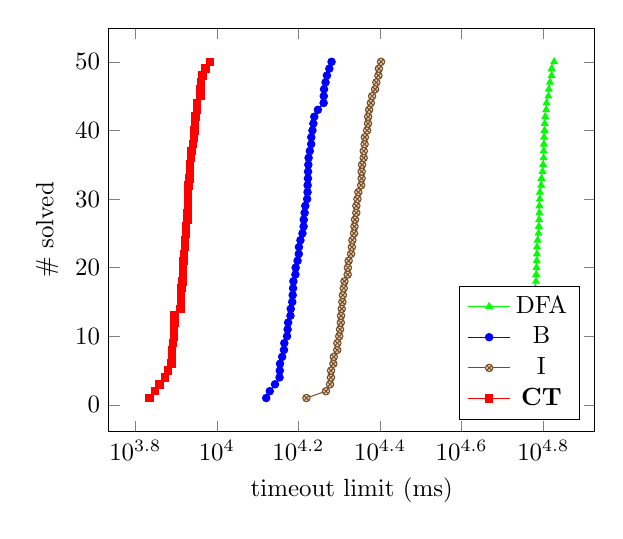
\begin{tikzpicture}[scale=0.9]
      \begin{axis}[
    xmode=log,
    every axis plot/.style={thin},
    xlabel={timeout limit (ms)},
    ylabel={\# solved},
    legend pos=south east
    % table/create on use/cumulative distribution/.style={
    %   create col/expr={\pgfmathaccuma + \thisrow{f(x)}}   
    % }
    ]
    \addplot 
    [mark=triangle*,
    mark size=1.5,
    mark options={solid},
    green] 
    coordinates {
    (51125.785, 1)
(54263.257, 2)
(56487.527, 3)
(56702.786, 4)
(56985.792, 5)
(57276.885, 6)
(57622.584, 7)
(58132.270, 8)
(58140.300, 9)
(58355.175, 10)
(58676.203, 11)
(59158.883, 12)
(59632.816, 13)
(59713.900, 14)
(59728.215, 15)
(60269.934, 16)
(60313.648, 17)
(60549.505, 18)
(60622.637, 19)
(60711.449, 20)
(60810.980, 21)
(60862.784, 22)
(60914.293, 23)
(61100.454, 24)
(61428.994, 25)
(61523.477, 26)
(61625.366, 27)
(61712.915, 28)
(61729.236, 29)
(61886.596, 30)
(61900.845, 31)
(62341.893, 32)
(62455.546, 33)
(62817.572, 34)
(63010.646, 35)
(63184.232, 36)
(63221.376, 37)
(63304.994, 38)
(63379.424, 39)
(63540.272, 40)
(63613.419, 41)
(63781.589, 42)
(64128.455, 43)
(64263.902, 44)
(64924.220, 45)
(65113.900, 46)
(65508.695, 47)
(66133.866, 48)
(66157.482, 49)
(67076.860, 50)
    };

    \addplot 
    [blue,
    mark=*,
    mark size=1.5,
    mark options={solid}]
    coordinates {
    (13210.645, 1)
(13478.699, 2)
(13880.904, 3)
(14240.906, 4)
(14262.586, 5)
(14281.012, 6)
(14453.879, 7)
(14601.257, 8)
(14630.915, 9)
(14856.229, 10)
(14906.587, 11)
(14947.426, 12)
(15147.432, 13)
(15173.599, 14)
(15300.351, 15)
(15338.350, 16)
(15370.471, 17)
(15400.162, 18)
(15575.398, 19)
(15599.555, 20)
(15767.367, 21)
(15876.487, 22)
(15890.540, 23)
(16026.936, 24)
(16207.081, 25)
(16313.213, 26)
(16328.178, 27)
(16410.911, 28)
(16468.425, 29)
(16641.910, 30)
(16678.794, 31)
(16689.212, 32)
(16716.749, 33)
(16728.322, 34)
(16755.929, 35)
(16780.814, 36)
(16896.779, 37)
(17026.619, 38)
(17037.921, 39)
(17147.387, 40)
(17237.324, 41)
(17326.549, 42)
(17685.575, 43)
(18266.956, 44)
(18281.157, 45)
(18310.293, 46)
(18466.165, 47)
(18608.783, 48)
(18864.433, 49)
(19102.683, 50)
    };

    \addplot [brown!60!black,
    mark options={fill=brown!40},
    mark=otimes*,
    mark size=1.5]
    coordinates {
    (16575.843, 1)
(18505.000, 2)
(18940.008, 3)
(19038.980, 4)
(19049.304, 5)
(19298.221, 6)
(19348.596, 7)
(19719.698, 8)
(19737.753, 9)
(19947.661, 10)
(20036.932, 11)
(20122.714, 12)
(20152.397, 13)
(20232.116, 14)
(20302.198, 15)
(20360.843, 16)
(20458.853, 17)
(20543.247, 18)
(20924.864, 19)
(20941.580, 20)
(21033.055, 21)
(21323.434, 22)
(21424.912, 23)
(21488.205, 24)
(21690.524, 25)
(21732.563, 26)
(21805.424, 27)
(21961.943, 28)
(21968.175, 29)
(22103.640, 30)
(22217.515, 31)
(22576.655, 32)
(22629.332, 33)
(22640.426, 34)
(22690.290, 35)
(22898.044, 36)
(22906.588, 37)
(23018.632, 38)
(23049.661, 39)
(23346.986, 40)
(23464.371, 41)
(23482.242, 42)
(23611.320, 43)
(23844.593, 44)
(24011.531, 45)
(24420.146, 46)
(24590.635, 47)
(24882.878, 48)
(24954.062, 49)
(25252.813, 50)
    };

    \addplot 
    [red,
    mark size=1.5,
    mark=square*]
    coordinates {
    (6834.272, 1)
(7049.566, 2)
(7238.120, 3)
(7457.754, 4)
(7598.772, 5)
(7739.737, 6)
(7771.586, 7)
(7772.970, 8)
(7812.433, 9)
(7861.439, 10)
(7862.003, 11)
(7867.552, 12)
(7871.233, 13)
(8146.006, 14)
(8162.853, 15)
(8169.022, 16)
(8197.217, 17)
(8246.900, 18)
(8258.157, 19)
(8262.374, 20)
(8291.516, 21)
(8318.251, 22)
(8342.451, 23)
(8355.561, 24)
(8389.425, 25)
(8401.690, 26)
(8470.665, 27)
(8475.034, 28)
(8489.871, 29)
(8495.761, 30)
(8507.506, 31)
(8510.152, 32)
(8560.945, 33)
(8587.622, 34)
(8588.072, 35)
(8642.789, 36)
(8662.209, 37)
(8738.285, 38)
(8798.802, 39)
(8820.422, 40)
(8831.432, 41)
(8851.771, 42)
(8928.438, 43)
(8949.293, 44)
(9107.856, 45)
(9118.812, 46)
(9135.516, 47)
(9225.896, 48)
(9370.806, 49)
(9607.234, 50)
    };
    \legend{DFA,B,I,\textbf{CT}}
  \end{axis}

    \end{tikzpicture}
    \vfill
    \caption{\textbf{A5}.}
    \vspace{\baselineskip}
  \end{minipage}\qquad
  \begin{minipage}[b][10cm][s]{0.45\textwidth}
    \centering
    \vfill
    \begin{tikzpicture}[scale=0.9]
      \begin{axis}[
    xmode=log,
    every axis plot/.style={thin},
    xlabel={timeout limit (ms)},
    ylabel={\% solved},
    legend style={at={(0.5,-0.30)},
      anchor=north,legend columns=-1},
    % legend pos=south east,
    cycle list/Set1-6,
            % define fill color for the marker
            mark list fill={.!75!white},
            mark options={solid,scale=0.9},
            cycle multiindex* list={
                Set1-6
                    \nextlist
                [3 of]linestyles
                    \nextlist
                very thick
                \nextlist
                mark=o,
                mark=*,
                mark=square,
                mark=triangle,
                mark=+
            },
    ]

    \addplot
    coordinates {

    };
    \addplot
    coordinates {
      (218870, 2)
      (301170, 4)
      (482210, 6)
      (553150, 8)
      (794860, 10)

    };
    \addplot
    coordinates {
      (296190, 2)
      (404230, 4)
      (606290, 6)
      (680520, 8)

    };
    \addplot
    coordinates {
      (15250, 2)
      (31320, 4)
      (36930, 6)
      (44950, 8)
      (48590, 10)
      (84800, 12)
      (105320, 15)
      (122290, 16)
      (149390, 18)
      (190110, 20)
      (199080, 22)
      (203260, 24)
      (205030, 26)
      (294700, 29)
      (410490, 30)
      (517330, 32)
      (796770, 34)

    };


    \legend{ B, I, \textbf{CT} }
  \end{axis}

    \end{tikzpicture}
    \vfill
    \caption{\textbf{A10}.}
    \vspace{\baselineskip}
  \end{minipage}\qquad
\end{figure}

\begin{figure}
  \begin{minipage}[b][10cm][s]{0.45\textwidth}
    \centering
    \vfill
    \begin{tikzpicture}[scale=0.9]
      \begin{axis}[
    xmode=log,
    every axis plot/.style={thin},
    xlabel={timeout limit (ms)},
    ylabel={\% solved},
    legend pos=south east,
    cycle list/Set1-6,
            % define fill color for the marker
            mark list fill={.!75!white},
            mark options={solid},
            cycle multiindex* list={
                Set1-6
                    \nextlist
                [3 of]linestyles
                    \nextlist
                very thick
                \nextlist
                mark=o,
                mark=*,
                mark=square,
                mark=triangle,
                mark=+
            },
    ]

    \addplot
    coordinates {
      (663310, 3)
      (668120, 6)
      (674240, 9)
      (681210, 12)
      (682080, 15)
      (693360, 18)
      (701800, 20)
      (710510, 23)
      (721370, 26)
      (733270, 29)
      (737690, 32)
      (743100, 35)
      (744950, 38)
      (746390, 40)
      (747580, 43)
      (747780, 46)
      (749520, 49)
      (752380, 52)
      (752460, 55)
      (752970, 58)
      (756240, 60)
      (756590, 63)
      (757070, 66)
      (757940, 69)
      (757950, 72)
      (758210, 75)
      (760950, 78)
      (761150, 80)
      (761270, 83)
      (762350, 86)
      (764150, 89)
      (764630, 92)
      (766660, 95)
      (778590, 98)
      (779820, 100)
      
    };
    \addplot
    coordinates {
      (48960, 3)
      (50130, 6)
      (50220, 9)
      (51730, 12)
      (52950, 15)
      (53810, 18)
      (78780, 20)
      (117310, 23)
      (204580, 26)
      (211480, 29)
      (211610, 32)
      (214100, 35)
      (218950, 38)
      (219710, 40)
      (221560, 43)
      (223130, 46)
      (225000, 49)
      (225250, 52)
      (226390, 55)
      (228770, 58)
      (228800, 60)
      (229210, 63)
      (229280, 66)
      (230400, 69)
      (230980, 72)
      (232150, 78)
      (236310, 80)
      (236880, 83)
      (237290, 86)
      (237320, 89)
      (238430, 92)
      (242000, 95)
      (247080, 98)
      (259880, 100)
      
    };
    \addplot
    coordinates {
      (48610, 3)
      (49700, 6)
      (49990, 9)
      (50810, 12)
      (51050, 15)
      (53250, 18)
      (90540, 20)
      (142650, 23)
      (275900, 26)
      (280260, 29)
      (282090, 32)
      (283200, 35)
      (283420, 38)
      (285910, 40)
      (287700, 43)
      (288220, 46)
      (291090, 49)
      (291560, 52)
      (294120, 55)
      (297560, 58)
      (297750, 60)
      (299160, 63)
      (300220, 66)
      (300620, 69)
      (301270, 72)
      (304330, 75)
      (308970, 78)
      (310620, 80)
      (310750, 83)
      (310990, 86)
      (311140, 89)
      (315640, 92)
      (328920, 95)
      (329910, 98)
      (341360, 100)
      
    };
    \addplot
    coordinates {
      (53490, 3)
      (54330, 6)
      (54840, 9)
      (55390, 12)
      (55780, 15)
      (56350, 18)
      (62080, 20)
      (76760, 23)
      (89920, 26)
      (92730, 29)
      (93300, 32)
      (93750, 35)
      (93760, 38)
      (93770, 40)
      (93910, 43)
      (94080, 46)
      (94190, 49)
      (94750, 52)
      (95060, 55)
      (95240, 58)
      (95480, 60)
      (95620, 63)
      (95790, 66)
      (95950, 69)
      (96350, 72)
      (96460, 78)
      (97070, 80)
      (97530, 83)
      (98260, 86)
      (98700, 89)
      (99170, 92)
      (99350, 95)
      (99830, 98)
      (100100, 100)
      
    };
    

    \legend{ DFA, B, I, \textbf{CT} }
  \end{axis}

    \end{tikzpicture}
    \vfill
    \caption{\textbf{BDD Large}.}
    \vspace{\baselineskip}
  \end{minipage}\qquad
  \begin{minipage}[b][10cm][s]{0.45\textwidth}
    \centering
    \vfill
    \begin{tikzpicture}[scale=0.9]
      \begin{axis}[
    xmode=log,
    every axis plot/.style={thin},
    xlabel={timeout limit (ms)},
    ylabel={\% solved},
    legend style={at={(0.5,-0.30)},
      anchor=north,legend columns=-1},
    % legend pos=south east,
    cycle list/Set1-6,
            % define fill color for the marker
            mark list fill={.!75!white},
            mark options={solid,scale=0.9},
            cycle multiindex* list={
                Set1-6
                    \nextlist
                [3 of]linestyles
                    \nextlist
                very thick
                \nextlist
                mark=o,
                mark=*,
                mark=square,
                mark=triangle,
                mark=+
            },
    ]

    

    \legend{ DFA, B, I, \textbf{CT} }
  \end{axis}

    \end{tikzpicture}
    \vfill
    \caption{\textbf{BDD Small}.}
    \vspace{\baselineskip}
  \end{minipage}\qquad
\end{figure}


\clearpage

\begin{figure}
  
  \begin{minipage}[b][10cm][s]{0.45\textwidth}
    \centering
    \vfill
    \begin{tikzpicture}[scale=0.9]
      \begin{axis}[
    xmode=log,
    every axis plot/.style={thin},
    xlabel={timeout limit (ms)},
    ylabel={\% solved},
    legend pos=south east,
    cycle list/Set1-6,
            % define fill color for the marker
            mark list fill={.!75!white},
            mark options={solid},
            cycle multiindex* list={
                Set1-6
                    \nextlist
                [3 of]linestyles
                    \nextlist
                very thick
                \nextlist
                mark=o,
                mark=*,
                mark=square,
                mark=triangle,
                mark=+
            },
    ]

    \addplot
    coordinates {
      (2550, 34)
      (4320, 67)
      (7020, 100)
      
    };
    \addplot
    coordinates {
      (2410, 34)
      (4300, 67)
      (7300, 100)
      
    };
    \addplot
    coordinates {
      (3770, 34)
      (6470, 67)
      (11240, 100)
      
    };
    \addplot
    coordinates {
      (1950, 34)
      (2830, 67)
      (4690, 100)
      
    };
    

    \legend{ DFA, B, I, \textbf{CT} }
  \end{axis}

    \end{tikzpicture}
    \vfill
    \caption{\textbf{AIM-50}.}
    \vspace{\baselineskip}
  \end{minipage}\qquad
  \begin{minipage}[b][10cm][s]{0.45\textwidth}
    \centering
    \vfill
    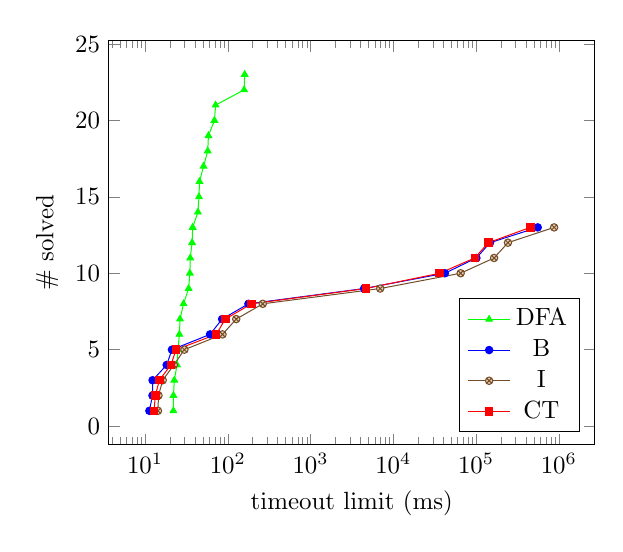
\begin{tikzpicture}[scale=0.9]
      \begin{axis}[
    xmode=log,
    every axis plot/.style={thin},
    xlabel={timeout limit (ms)},
    ylabel={\# solved},
    legend pos=south east
    % table/create on use/cumulative distribution/.style={
    %   create col/expr={\pgfmathaccuma + \thisrow{f(x)}}   
    % }
    ]
    \addplot 
    [mark=triangle*,
    mark size=1.5,
    mark options={solid},
    green] 
    coordinates {
    (21.989, 1)
(22.041, 2)
(22.559, 3)
(24.331, 4)
(24.974, 5)
(26.007, 6)
(26.462, 7)
(29.157, 8)
(33.602, 9)
(34.800, 10)
(35.158, 11)
(37.017, 12)
(37.604, 13)
(43.531, 14)
(44.847, 15)
(45.476, 16)
(50.917, 17)
(57.169, 18)
(58.349, 19)
(68.896, 20)
(71.202, 21)
(157.413, 22)
(159.802, 23)
    };

    \addplot 
    [blue,
    mark=*,
    mark size=1.5,
    mark options={solid}]
    coordinates {
    (11.281, 1)
(12.293, 2)
(12.323, 3)
(18.245, 4)
(21.125, 5)
(61.006, 6)
(85.311, 7)
(177.463, 8)
(4439.520, 9)
(41952.782, 10)
(100937.940, 11)
(147496.534, 12)
(556008.284, 13)
% (1000003.406, 14)
% (1000003.522, 15)
% (1000003.551, 16)
% (1000003.690, 17)
% (1000003.713, 18)
% (1000003.866, 19)
% (1000003.877, 20)
% (1000004.136, 21)
% (1000004.172, 22)
% (1000004.261, 23)
    };

    \addplot [brown!60!black,
    mark options={fill=brown!40},
    mark=otimes*,
    mark size=1.5]
    coordinates {
    (14.319, 1)
(14.525, 2)
(16.358, 3)
(22.251, 4)
(29.907, 5)
(86.300, 6)
(126.361, 7)
(264.396, 8)
(6937.110, 9)
(65105.320, 10)
(165084.246, 11)
(242777.983, 12)
(877449.095, 13)
% (1000004.285, 14)
% (1000004.482, 15)
% (1000004.500, 16)
% (1000004.632, 17)
% (1000004.858, 18)
% (1000004.869, 19)
% (1000004.994, 20)
% (1000015.307, 21)
% (1000021.218, 22)
% (1000094.474, 23)
    };

    \addplot 
    [red,
    mark size=1.5,
    mark=square*]
    coordinates {
    (12.839, 1)
(13.309, 2)
(14.887, 3)
(20.483, 4)
(23.742, 5)
(72.390, 6)
(93.185, 7)
(193.329, 8)
(4643.160, 9)
(36315.326, 10)
(96472.476, 11)
(140766.972, 12)
(452413.350, 13)
% (1000004.885, 14)
% (1000005.183, 15)
% (1000005.227, 16)
% (1000005.436, 17)
% (1000005.455, 18)
% (1000005.543, 19)
% (1000009.510, 20)
% (1000018.333, 21)
% (1000020.654, 22)
% (1000126.631, 23)
    };
    \legend{DFA,B,I,CT}
  \end{axis}

    \end{tikzpicture}
    \vfill
    \caption{\textbf{AIM-100}.}
    \vspace{\baselineskip}
  \end{minipage}\qquad
\end{figure}

\begin{figure}
  \begin{minipage}[b][10cm][s]{0.45\textwidth}
    \centering
    \vfill
    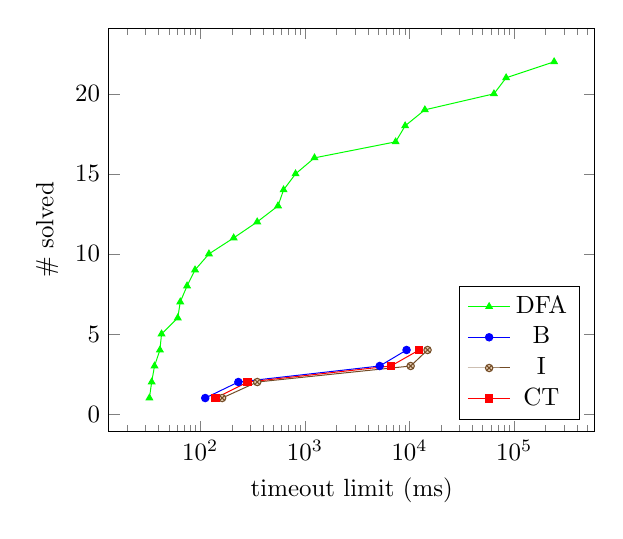
\begin{tikzpicture}[scale=0.9]
      \begin{axis}[
    xmode=log,
    every axis plot/.style={thin},
    xlabel={timeout limit (ms)},
    ylabel={\# solved},
    legend pos=south east
    % table/create on use/cumulative distribution/.style={
    %   create col/expr={\pgfmathaccuma + \thisrow{f(x)}}   
    % }
    ]
    \addplot 
    [mark=triangle*,
    mark size=1.5,
    mark options={solid},
    green] 
    coordinates {
    (32.646, 1)
(34.322, 2)
(36.539, 3)
(41.139, 4)
(42.637, 5)
(60.923, 6)
(64.362, 7)
(74.768, 8)
(89.108, 9)
(121.012, 10)
(208.525, 11)
(350.032, 12)
(553.291, 13)
(625.153, 14)
(813.725, 15)
(1234.205, 16)
(7361.018, 17)
(9076.992, 18)
(14005.709, 19)
(64038.325, 20)
(83738.459, 21)
(240798.763, 22)
    };

    \addplot 
    [blue,
    mark=*,
    mark size=1.5,
    mark options={solid}]
    coordinates {
    (111.532, 1)
(231.223, 2)
(5185.609, 3)
(9363.587, 4)
% (1000006.135, 5)
% (1000006.157, 6)
% (1000006.188, 7)
% (1000006.300, 8)
% (1000006.306, 9)
% (1000007.024, 10)
% (1000007.087, 11)
% (1000007.302, 12)
% (1000007.563, 13)
% (1000010.560, 14)
% (1000010.850, 15)
% (1000046.435, 16)
% (1000167.771, 17)
% (1001173.564, 18)
% (1006453.700, 19)
% (1008543.597, 20)
% (1010562.071, 21)
% (1019241.202, 22)
    };

    \addplot [brown!60!black,
    mark options={fill=brown!40},
    mark=otimes*,
    mark size=1.5]
    coordinates {
    (161.801, 1)
(350.376, 2)
(10244.105, 3)
(14856.666, 4)
% (1000007.483, 5)
% (1000007.625, 6)
% (1000007.695, 7)
% (1000008.729, 8)
% (1000009.950, 9)
% (1000011.262, 10)
% (1000019.536, 11)
% (1000023.192, 12)
% (1000025.767, 13)
% (1000040.365, 14)
% (1000041.636, 15)
% (1000051.012, 16)
% (1000053.849, 17)
% (1000118.768, 18)
% (1000166.508, 19)
% (1000467.387, 20)
% (1001776.595, 21)
% (1015356.678, 22)
    };

    \addplot 
    [red,
    mark size=1.5,
    mark=square*]
    coordinates {
    (140.045, 1)
(284.098, 2)
(6638.875, 3)
(12352.151, 4)
% (1000007.437, 5)
% (1000007.976, 6)
% (1000009.059, 7)
% (1000009.398, 8)
% (1000009.787, 9)
% (1000013.785, 10)
% (1000024.236, 11)
% (1000038.306, 12)
% (1000061.649, 13)
% (1000067.115, 14)
% (1000073.775, 15)
% (1000110.045, 16)
% (1000202.940, 17)
% (1000283.824, 18)
% (1001241.998, 19)
% (1012931.719, 20)
% (1016410.000, 21)
% (1021392.559, 22)
    };
    \legend{DFA,B,I,CT}
  \end{axis}

    \end{tikzpicture}
    \vfill
    \caption{\textbf{AIM-200}.}
    \vspace{\baselineskip}
  \end{minipage}\qquad
\end{figure}


\clearpage

\begin{figure}
  \begin{minipage}[b][10cm][s]{0.45\textwidth}
    \centering
    \vfill
    \begin{tikzpicture}[scale=0.9]
      \begin{axis}[
    xmode=log,
    every axis plot/.style={thin},
    xlabel={timeout limit (ms)},
    ylabel={\% solved},
    legend style={at={(0.5,-0.30)},
      anchor=north,legend columns=-1},
    % legend pos=south east,
    cycle list/Set1-6,
            % define fill color for the marker
            mark list fill={.!75!white},
            mark options={solid,scale=0.9},
            cycle multiindex* list={
                Set1-6
                    \nextlist
                [3 of]linestyles
                    \nextlist
                very thick
                \nextlist
                mark=o,
                mark=*,
                mark=square,
                mark=triangle,
                mark=+
            },
    ]

    \addplot
    coordinates {
      (1090, 3)
      (1130, 5)
      (1340, 7)
      (1460, 9)
      (1550, 11)
      (1590, 14)
      (1680, 16)
      (1880, 18)
      (2240, 20)
      (2320, 22)
      (2340, 24)
      (2450, 27)
      (2830, 29)
      (3190, 31)
      (3290, 33)
      (3500, 35)
      (3550, 37)
      (3870, 40)
      (4340, 42)
      (4350, 44)
      (4680, 46)
      (4950, 48)
      (5270, 50)
      (5400, 53)
      (5880, 55)
      (6280, 57)
      (6960, 59)
      (8170, 61)
      (8770, 64)
      (9380, 66)
      (9840, 68)
      (13500, 70)
      (17400, 72)
      (22580, 74)
      (23570, 77)
      (23810, 79)
      (33320, 81)
      (67210, 83)
      (75510, 85)
      (79890, 87)
      (94840, 90)
      (99880, 92)
      (118040, 94)
      (145590, 96)
      (146260, 98)
      (252130, 100)
      
    };
    \addplot
    coordinates {
      (40, 3)
      (50, 5)
      (60, 11)
      (70, 14)
      (80, 16)
      (90, 22)
      (120, 27)
      (130, 29)
      (170, 31)
      (180, 33)
      (190, 35)
      (300, 37)
      (310, 40)
      (450, 42)
      (540, 44)
      (590, 46)
      (890, 48)
      (930, 50)
      (1310, 53)
      (1560, 55)
      (2010, 57)
      (3940, 59)
      (5330, 61)
      (5390, 64)
      (7080, 66)
      (8650, 68)
      (11800, 70)
      (21010, 72)
      (36960, 74)
      (42090, 77)
      (52930, 79)
      (70600, 81)
      (140070, 83)
      (219890, 85)
      (259150, 87)
      (290930, 90)
      (293180, 92)
      (307460, 94)
      (415600, 96)
      (417390, 98)
      (879060, 100)
      
    };
    \addplot
    coordinates {
      (50, 5)
      (60, 9)
      (70, 11)
      (80, 14)
      (90, 20)
      (100, 22)
      (130, 27)
      (150, 29)
      (220, 35)
      (410, 37)
      (450, 40)
      (490, 42)
      (730, 44)
      (890, 46)
      (1130, 48)
      (1400, 50)
      (1810, 53)
      (2220, 55)
      (2740, 57)
      (5190, 59)
      (6980, 61)
      (7220, 64)
      (8240, 66)
      (11030, 68)
      (15130, 70)
      (26310, 72)
      (45850, 74)
      (51450, 77)
      (65270, 79)
      (80850, 81)
      (169630, 83)
      (259520, 85)
      (311430, 87)
      (346140, 90)
      (353150, 92)
      (361750, 94)
      (492850, 96)
      (494920, 98)
      
    };
    \addplot
    coordinates {
      (50, 3)
      (60, 7)
      (70, 11)
      (80, 14)
      (90, 20)
      (100, 22)
      (120, 24)
      (130, 29)
      (140, 33)
      (160, 35)
      (180, 37)
      (200, 42)
      (210, 44)
      (290, 48)
      (350, 50)
      (410, 53)
      (490, 55)
      (500, 57)
      (750, 59)
      (870, 61)
      (950, 64)
      (1000, 66)
      (1450, 68)
      (1840, 70)
      (3040, 72)
      (5480, 74)
      (6280, 77)
      (6480, 79)
      (6970, 81)
      (16740, 83)
      (26310, 85)
      (28910, 87)
      (29020, 90)
      (33910, 92)
      (36940, 94)
      (45410, 96)
      (50170, 98)
      (97580, 100)
      
    };
    

    \legend{ DFA, B, I, \textbf{CT} }
  \end{axis}

    \end{tikzpicture}
    \vfill
    \caption{\textbf{Crosswords WorldVG}.}
    \vspace{\baselineskip}
  \end{minipage}\qquad
  \begin{minipage}[b][10cm][s]{0.45\textwidth}
    \centering
    \vfill
    \begin{tikzpicture}[scale=0.9]
      \begin{axis}[
    xmode=log,
    every axis plot/.style={thin},
    xlabel={timeout limit (ms)},
    ylabel={\% solved},
    legend style={at={(0.5,-0.30)},
      anchor=north,legend columns=-1},
    % legend pos=south east,
    cycle list/Set1-6,
            % define fill color for the marker
            mark list fill={.!75!white},
            mark options={solid,scale=0.9},
            cycle multiindex* list={
                Set1-6
                    \nextlist
                [3 of]linestyles
                    \nextlist
                very thick
                \nextlist
                mark=o,
                mark=*,
                mark=square,
                mark=triangle,
                mark=+
            },
    ]

    \addplot
    coordinates {
      (1070, 3)
      (1090, 6)
      (1100, 9)
      (1140, 12)
      (1340, 15)
      (1620, 18)
      (1650, 20)
      (1780, 23)
      (1830, 26)
      (2280, 29)
      (2300, 32)
      (2340, 35)
      (2490, 38)
      (2750, 40)
      (2880, 43)
      (3070, 46)
      (3780, 49)
      (3960, 52)
      (4590, 55)
      (4680, 58)
      (4980, 60)
      (5180, 63)
      (5480, 66)
      (8310, 69)
      (11060, 72)
      (11440, 75)
      (14310, 78)
      (15080, 80)
      (23840, 83)
      (28160, 86)
      (34450, 89)
      (35060, 92)
      (45870, 95)
      (49120, 98)
      (62030, 100)
      
    };
    \addplot
    coordinates {
      (50, 6)
      (60, 9)
      (70, 12)
      (80, 18)
      (130, 23)
      (200, 26)
      (240, 29)
      (330, 32)
      (360, 35)
      (840, 38)
      (1000, 40)
      (1340, 43)
      (1420, 46)
      (1570, 49)
      (2440, 52)
      (2810, 55)
      (4430, 58)
      (5330, 60)
      (7350, 63)
      (7450, 66)
      (12850, 69)
      (16490, 72)
      (19310, 75)
      (20520, 78)
      (23670, 80)
      (39020, 83)
      (62930, 86)
      (65710, 89)
      (70870, 92)
      (109260, 95)
      (117110, 98)
      (144570, 100)
      
    };
    \addplot
    coordinates {
      (50, 6)
      (70, 12)
      (100, 18)
      (170, 20)
      (190, 23)
      (300, 26)
      (320, 29)
      (500, 35)
      (1120, 38)
      (1330, 40)
      (1630, 43)
      (1720, 46)
      (2180, 49)
      (3200, 52)
      (3680, 55)
      (5710, 58)
      (6810, 60)
      (9230, 63)
      (9390, 66)
      (16190, 69)
      (18960, 72)
      (24090, 75)
      (25580, 78)
      (29300, 80)
      (47970, 83)
      (75460, 86)
      (80010, 89)
      (85710, 92)
      (129810, 95)
      (138470, 98)
      (170370, 100)
      
    };
    \addplot
    coordinates {
      (50, 6)
      (60, 9)
      (70, 12)
      (80, 18)
      (100, 20)
      (110, 26)
      (140, 29)
      (160, 32)
      (180, 35)
      (230, 38)
      (240, 40)
      (260, 43)
      (300, 46)
      (440, 49)
      (520, 52)
      (580, 55)
      (820, 58)
      (970, 60)
      (1270, 63)
      (1290, 66)
      (2040, 69)
      (2350, 72)
      (3050, 75)
      (3340, 78)
      (3870, 80)
      (6030, 83)
      (10650, 86)
      (10890, 89)
      (11130, 92)
      (14780, 95)
      (20090, 98)
      (24080, 100)
      
    };
    

    \legend{ DFA, B, I, \textbf{CT} }
  \end{axis}

    \end{tikzpicture}
    \vfill
    \caption{\textbf{Crosswords LexVG}.}
    \vspace{\baselineskip}
  \end{minipage}\qquad
\end{figure}

\begin{figure}
  \begin{minipage}[b][10cm][s]{0.45\textwidth}
    \centering
    \vfill
    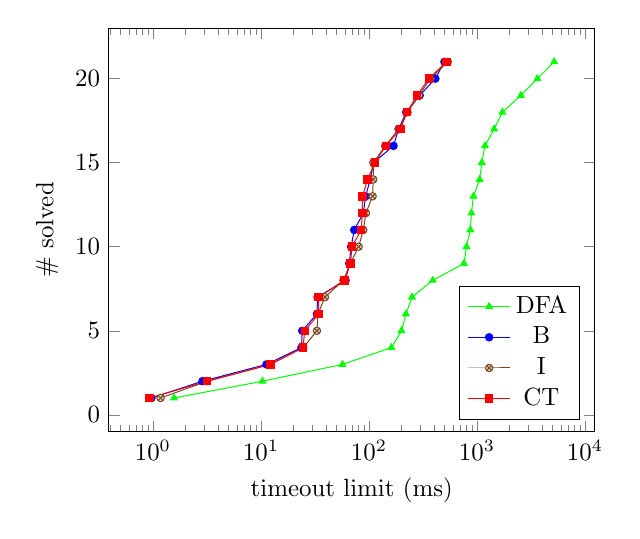
\begin{tikzpicture}[scale=0.9]
      \begin{axis}[
    xmode=log,
    every axis plot/.style={thin},
    xlabel={timeout limit (ms)},
    ylabel={\# solved},
    legend pos=south east
    % table/create on use/cumulative distribution/.style={
    %   create col/expr={\pgfmathaccuma + \thisrow{f(x)}}   
    % }
    ]
    \addplot 
    [mark=triangle*,
    mark size=1.5,
    mark options={solid},
    green] 
    coordinates {
(1.569, 1)
(10.341, 2)
(56.930, 3)
(161.466, 4)
(200.271, 5)
(220.150, 6)
(250.496, 7)
(389.479, 8)
(757.830, 9)
(800.580, 10)
(868.873, 11)
(888.415, 12)
(928.329, 13)
(1059.826, 14)
(1108.592, 15)
(1186.171, 16)
(1442.143, 17)
(1718.117, 18)
(2549.019, 19)
(3626.036, 20)
(5178.601, 21)
    };

    \addplot 
    [blue,
    mark=*,
    mark size=1.5,
    mark options={solid}]
    coordinates {
(0.969, 1)
(2.881, 2)
(11.268, 3)
(23.734, 4)
(24.138, 5)
(33.016, 6)
(33.480, 7)
(60.819, 8)
(65.730, 9)
(68.464, 10)
(73.136, 11)
(88.944, 12)
(92.941, 13)
(103.030, 14)
(110.307, 15)
(168.815, 16)
(188.304, 17)
(221.341, 18)
(295.291, 19)
(412.154, 20)
(499.695, 21)
    };

    \addplot [brown!60!black,
    mark options={fill=brown!40},
    mark=otimes*,
    mark size=1.5]
    coordinates {
(1.178, 1)
(3.182, 2)
(12.190, 3)
(24.682, 4)
(33.012, 5)
(33.778, 6)
(39.197, 7)
(58.045, 8)
(67.182, 9)
(80.311, 10)
(88.742, 11)
(93.862, 12)
(108.193, 13)
(109.575, 14)
(110.207, 15)
(141.416, 16)
(189.383, 17)
(227.490, 18)
(289.981, 19)
(370.487, 20)
(537.222, 21)
    };

    \addplot 
    [red,
    mark size=1.5,
    mark=square*]
    coordinates {
(0.929, 1)
(3.171, 2)
(12.289, 3)
(24.504, 4)
(25.467, 5)
(34.223, 6)
(34.294, 7)
(59.192, 8)
(67.660, 9)
(69.445, 10)
(84.905, 11)
(86.923, 12)
(87.166, 13)
(97.317, 14)
(113.314, 15)
(143.394, 16)
(195.333, 17)
(225.252, 18)
(279.125, 19)
(358.324, 20)
(525.028, 21)
    };
    \legend{DFA,B,I,CT}
  \end{axis}

    \end{tikzpicture}
    \vfill
    \caption{\textbf{Crosswords Wordspuzzle}.}
    \vspace{\baselineskip}
  \end{minipage}\qquad
\end{figure}


\clearpage

\begin{figure}
  \begin{minipage}[b][10cm][s]{0.45\textwidth}
    \centering
    \vfill
    \begin{tikzpicture}[scale=0.9]
      \begin{axis}[
    xmode=log,
    every axis plot/.style={thin},
    xlabel={timeout limit (ms)},
    ylabel={\% solved},
    legend pos=south east,
    cycle list/Set1-6,
            % define fill color for the marker
            mark list fill={.!75!white},
            mark options={solid},
            cycle multiindex* list={
                Set1-6
                    \nextlist
                [3 of]linestyles
                    \nextlist
                very thick
                \nextlist
                mark=o,
                mark=*,
                mark=square,
                mark=triangle,
                mark=+
            },
    ]

    \addplot
    coordinates {
      (221050, 50)
      
    };
    \addplot
    coordinates {
      (215740, 50)
      
    };
    \addplot
    coordinates {
      (286600, 50)
      
    };
    \addplot
    coordinates {
      (198370, 50)
      
    };
    

    \legend{ DFA, B, I, \textbf{CT} }
  \end{axis}

    \end{tikzpicture}
    \vfill
    \caption{\textbf{Dubois}.}
    \vspace{\baselineskip}
  \end{minipage}\qquad
  \begin{minipage}[b][10cm][s]{0.45\textwidth}
    \centering
    \vfill
    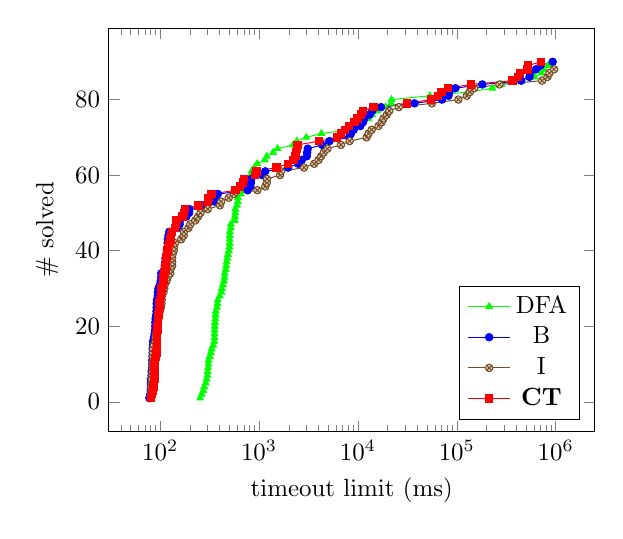
\begin{tikzpicture}[scale=0.9]
      \begin{axis}[
    xmode=log,
    every axis plot/.style={thin},
    xlabel={timeout limit (ms)},
    ylabel={\# solved},
    legend pos=south east
    % table/create on use/cumulative distribution/.style={
    %   create col/expr={\pgfmathaccuma + \thisrow{f(x)}}   
    % }
    ]
    \addplot 
    [mark=triangle*,
    mark size=1.5,
    mark options={solid},
    green] 
    coordinates {
(253.940, 1)
(262.899, 2)
(272.809, 3)
(278.671, 4)
(288.456, 5)
(294.738, 6)
(300.533, 7)
(301.856, 8)
(305.317, 9)
(307.585, 10)
(307.747, 11)
(317.045, 12)
(325.386, 13)
(331.714, 14)
(343.719, 15)
(352.611, 16)
(354.157, 17)
(354.187, 18)
(355.194, 19)
(355.670, 20)
(358.353, 21)
(361.624, 22)
(363.056, 23)
(364.990, 24)
(375.254, 25)
(379.066, 26)
(381.267, 27)
(400.323, 28)
(416.524, 29)
(419.193, 30)
(431.537, 31)
(441.410, 32)
(446.582, 33)
(449.777, 34)
(459.308, 35)
(465.151, 36)
(469.990, 37)
(476.800, 38)
(483.769, 39)
(495.431, 40)
(499.645, 41)
(504.063, 42)
(504.308, 43)
(504.525, 44)
(505.961, 45)
(518.392, 46)
(518.507, 47)
(566.413, 48)
(568.752, 49)
(575.921, 50)
(576.168, 51)
(596.357, 52)
(608.960, 53)
(610.697, 54)
(655.605, 55)
(657.724, 56)
(659.099, 57)
(661.565, 58)
(793.731, 59)
(829.897, 60)
(838.681, 61)
(897.103, 62)
(955.465, 63)
(1140.095, 64)
(1197.349, 65)
(1386.206, 66)
(1532.332, 67)
(2202.746, 68)
(2405.914, 69)
(2998.076, 70)
(4263.504, 71)
(7966.854, 72)
(8986.821, 73)
(10565.606, 74)
(12775.906, 75)
(13934.651, 76)
(15637.959, 77)
(18950.571, 78)
(21686.565, 79)
(21854.085, 80)
(53338.868, 81)
(128675.786, 82)
(229123.808, 83)
(281459.430, 84)
(391898.437, 85)
(610230.975, 86)
(714999.649, 87)
(762531.311, 88)
(838054.743, 89)
    };

    \addplot 
    [blue,
    mark=*,
    mark size=1.5,
    mark options={solid}]
    coordinates {
(77.750, 1)
(79.361, 2)
(80.110, 3)
(80.478, 4)
(80.514, 5)
(80.733, 6)
(81.819, 7)
(81.865, 8)
(82.700, 9)
(83.055, 10)
(83.084, 11)
(83.660, 12)
(83.815, 13)
(83.884, 14)
(84.339, 15)
(84.779, 16)
(86.333, 17)
(87.672, 18)
(88.800, 19)
(89.170, 20)
(89.209, 21)
(89.917, 22)
(91.234, 23)
(91.710, 24)
(92.131, 25)
(92.191, 26)
(92.825, 27)
(94.385, 28)
(94.984, 29)
(95.858, 30)
(99.363, 31)
(101.208, 32)
(102.326, 33)
(102.457, 34)
(109.924, 35)
(111.293, 36)
(112.684, 37)
(113.090, 38)
(115.314, 39)
(117.192, 40)
(118.738, 41)
(118.994, 42)
(119.411, 43)
(121.235, 44)
(123.390, 45)
(150.523, 46)
(157.344, 47)
(158.315, 48)
(182.842, 49)
(196.164, 50)
(197.579, 51)
(277.635, 52)
(354.634, 53)
(359.251, 54)
(383.268, 55)
(766.566, 56)
(816.221, 57)
(827.832, 58)
(833.240, 59)
(1081.574, 60)
(1153.362, 61)
(1963.070, 62)
(2492.142, 63)
(2701.259, 64)
(3034.945, 65)
(3062.028, 66)
(3107.310, 67)
(4356.706, 68)
(5152.815, 69)
(8143.306, 70)
(8488.009, 71)
(9065.789, 72)
(10578.592, 73)
(11242.491, 74)
(11618.200, 75)
(13121.563, 76)
(13946.231, 77)
(17115.205, 78)
(37255.008, 79)
(70596.495, 80)
(82332.599, 81)
(83994.429, 82)
(96686.082, 83)
(180912.619, 84)
(447647.179, 85)
(543188.377, 86)
(549287.562, 87)
(631674.574, 88)
(702660.342, 89)
(931931.366, 90)
    };

    \addplot [brown!60!black,
    mark options={fill=brown!40},
    mark=otimes*,
    mark size=1.5]
    coordinates {
(80.607, 1)
(80.621, 2)
(81.289, 3)
(81.598, 4)
(81.969, 5)
(82.414, 6)
(83.447, 7)
(83.492, 8)
(83.796, 9)
(83.946, 10)
(84.672, 11)
(84.778, 12)
(84.834, 13)
(85.069, 14)
(86.207, 15)
(89.293, 16)
(89.663, 17)
(90.436, 18)
(92.701, 19)
(93.412, 20)
(95.453, 21)
(96.026, 22)
(97.734, 23)
(99.208, 24)
(101.597, 25)
(103.239, 26)
(103.380, 27)
(103.698, 28)
(107.856, 29)
(109.858, 30)
(111.092, 31)
(116.012, 32)
(119.197, 33)
(126.351, 34)
(126.923, 35)
(131.997, 36)
(132.037, 37)
(132.076, 38)
(133.087, 39)
(137.356, 40)
(137.793, 41)
(141.326, 42)
(162.716, 43)
(172.556, 44)
(173.424, 45)
(192.918, 46)
(201.428, 47)
(226.385, 48)
(241.352, 49)
(255.602, 50)
(302.351, 51)
(401.666, 52)
(413.952, 53)
(493.052, 54)
(555.383, 55)
(961.003, 56)
(1155.835, 57)
(1196.833, 58)
(1202.095, 59)
(1628.244, 60)
(1659.941, 61)
(2850.318, 62)
(3611.710, 63)
(3991.524, 64)
(4242.800, 65)
(4511.471, 66)
(4915.881, 67)
(6733.256, 68)
(8232.380, 69)
(12233.495, 70)
(12792.050, 71)
(13747.597, 72)
(16126.327, 73)
(17376.344, 74)
(18154.073, 75)
(19607.670, 76)
(20742.169, 77)
(25931.910, 78)
(55946.249, 79)
(103693.950, 80)
(126173.635, 81)
(135526.885, 82)
(149917.691, 83)
(270068.501, 84)
(727604.821, 85)
(825691.112, 86)
(863292.217, 87)
(964034.894, 88)
    };

    \addplot 
    [red,
    mark size=1.5,
    mark=square*]
    coordinates {
(80.539, 1)
(82.933, 2)
(84.502, 3)
(85.194, 4)
(86.750, 5)
(87.225, 6)
(87.348, 7)
(87.379, 8)
(87.590, 9)
(87.799, 10)
(89.072, 11)
(90.371, 12)
(91.497, 13)
(92.339, 14)
(92.677, 15)
(92.786, 16)
(92.837, 17)
(93.306, 18)
(94.022, 19)
(94.387, 20)
(94.732, 21)
(94.876, 22)
(95.771, 23)
(97.088, 24)
(97.931, 25)
(98.786, 26)
(99.264, 27)
(101.340, 28)
(102.067, 29)
(102.698, 30)
(106.996, 31)
(108.150, 32)
(108.319, 33)
(109.028, 34)
(112.687, 35)
(112.838, 36)
(113.987, 37)
(115.735, 38)
(116.607, 39)
(117.896, 40)
(120.281, 41)
(124.525, 42)
(127.605, 43)
(129.317, 44)
(131.451, 45)
(140.940, 46)
(144.202, 47)
(145.438, 48)
(168.774, 49)
(174.703, 50)
(178.916, 51)
(244.908, 52)
(305.799, 53)
(306.522, 54)
(329.051, 55)
(577.969, 56)
(639.964, 57)
(687.996, 58)
(705.323, 59)
(904.996, 60)
(941.051, 61)
(1495.517, 62)
(1970.419, 63)
(2227.812, 64)
(2340.143, 65)
(2350.643, 66)
(2430.290, 67)
(2443.247, 68)
(4040.442, 69)
(6139.544, 70)
(6717.200, 71)
(7384.930, 72)
(8139.677, 73)
(9195.984, 74)
(9860.741, 75)
(10763.986, 76)
(11275.949, 77)
(14355.361, 78)
(31179.882, 79)
(55057.738, 80)
(64542.114, 81)
(70093.034, 82)
(81511.901, 83)
(138808.782, 84)
(367231.073, 85)
(417571.146, 86)
(437364.064, 87)
(519365.523, 88)
(525638.664, 89)
(705868.408, 90)
    };
    \legend{DFA,B,I,\textbf{CT}}
  \end{axis}

    \end{tikzpicture}
    \vfill
    \caption{\textbf{Geom}.}
    \vspace{\baselineskip}
  \end{minipage}\qquad
\end{figure}

\begin{figure}
  \begin{minipage}[b][10cm][s]{0.45\textwidth}
    \centering
    \vfill
    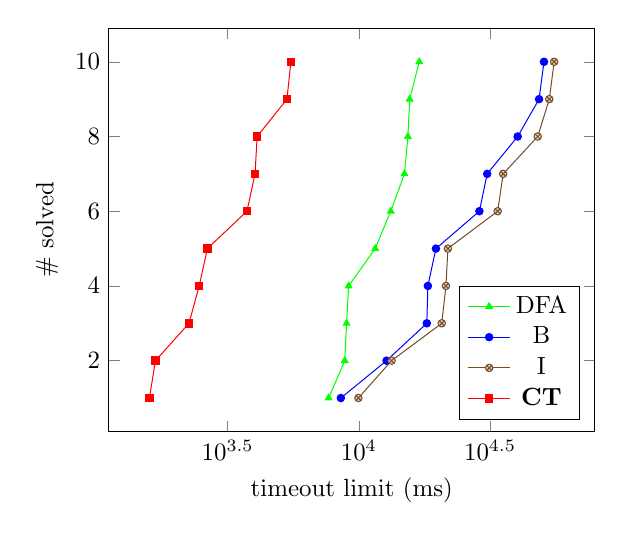
\begin{tikzpicture}[scale=0.9]
      \begin{axis}[
    xmode=log,
    every axis plot/.style={thin},
    xlabel={timeout limit (ms)},
    ylabel={\# solved},
    legend pos=south east
    % table/create on use/cumulative distribution/.style={
    %   create col/expr={\pgfmathaccuma + \thisrow{f(x)}}   
    % }
    ]
    \addplot 
    [mark=triangle*,
    mark size=1.5,
    mark options={solid},
    green] 
    coordinates {
    (7669.883, 1)
(8836.338, 2)
(8977.330, 3)
(9140.777, 4)
(11537.562, 5)
(13231.384, 6)
(14923.762, 7)
(15381.136, 8)
(15623.402, 9)
(16994.255, 10)
    };

    \addplot 
    [blue,
    mark=*,
    mark size=1.5,
    mark options={solid}]
    coordinates {
    (8538.228, 1)
(12749.685, 2)
(18156.956, 3)
(18327.323, 4)
(19669.292, 5)
(28802.590, 6)
(30835.715, 7)
(40301.654, 8)
(48620.995, 9)
(50774.009, 10)
    };

    \addplot [brown!60!black,
    mark options={fill=brown!40},
    mark=otimes*,
    mark size=1.5]
    coordinates {
    (9960.047, 1)
(13326.927, 2)
(20700.530, 3)
(21474.840, 4)
(21842.271, 5)
(33817.893, 6)
(35489.987, 7)
(48049.593, 8)
(53196.297, 9)
(55499.785, 10)
    };

    \addplot 
    [red,
    mark size=1.5,
    mark=square*]
    coordinates {
    (1591.239, 1)
(1678.457, 2)
(2251.773, 3)
(2462.919, 4)
(2646.514, 5)
(3745.993, 6)
(4020.526, 7)
(4095.836, 8)
(5320.617, 9)
(5507.353, 10)
    };
    \legend{DFA,B,I,\textbf{CT}}
  \end{axis}

    \end{tikzpicture}
    \vfill
    \caption{\textbf{K5}.}
    \vspace{\baselineskip}
  \end{minipage}\qquad
\end{figure}

\clearpage

\begin{figure}
  \begin{minipage}[b][10cm][s]{0.45\textwidth}
    \centering
    \vfill
    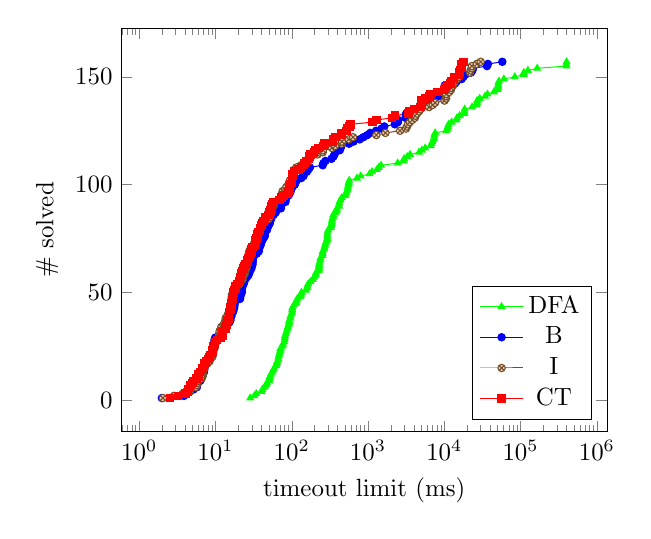
\begin{tikzpicture}[scale=0.9]
      \begin{axis}[
    xmode=log,
    every axis plot/.style={thin},
    xlabel={timeout limit (ms)},
    ylabel={\# solved},
    legend pos=south east
    % table/create on use/cumulative distribution/.style={
    %   create col/expr={\pgfmathaccuma + \thisrow{f(x)}}   
    % }
    ]
    \addplot 
    [mark=triangle*,
    mark size=1.5,
    mark options={solid},
    green] 
    coordinates {
    (28.479, 1)
(32.259, 2)
(34.184, 3)
(40.176, 4)
(41.117, 5)
(44.220, 6)
(46.524, 7)
(47.119, 8)
(50.594, 9)
(51.185, 10)
(51.683, 11)
(53.094, 12)
(55.381, 13)
(57.551, 14)
(58.822, 15)
(62.806, 16)
(64.164, 17)
(64.612, 18)
(66.816, 19)
(66.879, 20)
(68.064, 21)
(69.387, 22)
(70.958, 23)
(71.154, 24)
(74.896, 25)
(76.696, 26)
(79.628, 27)
(80.614, 28)
(80.994, 29)
(81.915, 30)
(83.799, 31)
(85.498, 32)
(87.376, 33)
(88.955, 34)
(90.775, 35)
(92.387, 36)
(92.399, 37)
(95.672, 38)
(96.038, 39)
(99.560, 40)
(101.063, 41)
(101.351, 42)
(102.343, 43)
(105.757, 44)
(114.544, 45)
(115.689, 46)
(117.793, 47)
(129.374, 48)
(131.156, 49)
(134.382, 50)
(152.723, 51)
(159.993, 52)
(160.432, 53)
(164.374, 54)
(176.218, 55)
(188.673, 56)
(197.819, 57)
(205.739, 58)
(207.344, 59)
(226.014, 60)
(227.529, 61)
(227.659, 62)
(227.801, 63)
(232.632, 64)
(236.122, 65)
(237.853, 66)
(253.358, 67)
(253.590, 68)
(254.330, 69)
(266.274, 70)
(268.730, 71)
(273.463, 72)
(277.735, 73)
(288.026, 74)
(291.548, 75)
(292.756, 76)
(293.227, 77)
(294.410, 78)
(300.709, 79)
(327.569, 80)
(332.541, 81)
(333.924, 82)
(334.411, 83)
(339.586, 84)
(348.199, 85)
(349.532, 86)
(371.373, 87)
(386.701, 88)
(390.963, 89)
(418.408, 90)
(418.695, 91)
(422.230, 92)
(437.503, 93)
(453.861, 94)
(502.971, 95)
(520.108, 96)
(527.304, 97)
(542.192, 98)
(544.013, 99)
(554.465, 100)
(558.086, 101)
(567.256, 102)
(715.556, 103)
(800.577, 104)
(1046.040, 105)
(1129.254, 106)
(1306.675, 107)
(1383.006, 108)
(1479.749, 109)
(2448.671, 110)
(2930.847, 111)
(2965.572, 112)
(3260.970, 113)
(3556.870, 114)
(4656.549, 115)
(5078.367, 116)
(5623.653, 117)
(6659.340, 118)
(6784.312, 119)
(6973.103, 120)
(7329.557, 121)
(7359.121, 122)
(7396.106, 123)
(7576.040, 124)
(10610.895, 125)
(10922.259, 126)
(11159.351, 127)
(11396.117, 128)
(12483.028, 129)
(14419.922, 130)
(14676.118, 131)
(15906.106, 132)
(18283.308, 133)
(18442.544, 134)
(18470.312, 135)
(23102.428, 136)
(26464.714, 137)
(26805.377, 138)
(26954.579, 139)
(29112.162, 140)
(34228.839, 141)
(36846.271, 142)
(44695.427, 143)
(50105.717, 144)
(50810.695, 145)
(50811.889, 146)
(51055.360, 147)
(51994.297, 148)
(60294.547, 149)
(83881.093, 150)
(110031.542, 151)
(110303.654, 152)
(124680.954, 153)
(164840.449, 154)
(398572.615, 155)
(398573.318, 156)
(401037.607, 157)
    };

    \addplot 
    [blue,
    mark=*,
    mark size=1.5,
    mark options={solid}]
    coordinates {
    (1.981, 1)
(3.865, 2)
(4.064, 3)
(4.147, 4)
(5.164, 5)
(5.702, 6)
(5.759, 7)
(5.839, 8)
(6.320, 9)
(6.503, 10)
(6.645, 11)
(6.804, 12)
(7.058, 13)
(7.115, 14)
(7.149, 15)
(7.349, 16)
(7.424, 17)
(7.744, 18)
(8.081, 19)
(8.255, 20)
(9.006, 21)
(9.029, 22)
(9.159, 23)
(9.557, 24)
(9.613, 25)
(9.675, 26)
(9.691, 27)
(9.705, 28)
(9.922, 29)
(11.049, 30)
(11.959, 31)
(12.363, 32)
(13.100, 33)
(13.492, 34)
(14.116, 35)
(15.142, 36)
(15.661, 37)
(15.767, 38)
(16.210, 39)
(16.247, 40)
(17.023, 41)
(17.310, 42)
(17.589, 43)
(17.712, 44)
(17.876, 45)
(18.383, 46)
(20.996, 47)
(21.124, 48)
(21.524, 49)
(22.126, 50)
(22.138, 51)
(22.244, 52)
(22.755, 53)
(23.472, 54)
(23.827, 55)
(24.361, 56)
(25.737, 57)
(27.024, 58)
(27.729, 59)
(28.322, 60)
(29.453, 61)
(30.020, 62)
(30.589, 63)
(30.689, 64)
(30.830, 65)
(31.200, 66)
(31.809, 67)
(34.778, 68)
(36.914, 69)
(36.958, 70)
(38.037, 71)
(39.151, 72)
(39.381, 73)
(40.922, 74)
(42.232, 75)
(44.223, 76)
(44.334, 77)
(44.614, 78)
(47.327, 79)
(47.856, 80)
(49.569, 81)
(51.504, 82)
(51.951, 83)
(53.451, 84)
(54.347, 85)
(57.828, 86)
(61.396, 87)
(63.159, 88)
(72.148, 89)
(72.466, 90)
(72.988, 91)
(82.727, 92)
(83.052, 93)
(85.267, 94)
(91.016, 95)
(94.242, 96)
(97.150, 97)
(97.576, 98)
(102.403, 99)
(109.460, 100)
(112.204, 101)
(115.663, 102)
(132.942, 103)
(142.599, 104)
(142.756, 105)
(158.121, 106)
(164.564, 107)
(173.027, 108)
(254.761, 109)
(260.341, 110)
(276.465, 111)
(331.631, 112)
(352.139, 113)
(362.559, 114)
(375.144, 115)
(427.109, 116)
(436.286, 117)
(447.651, 118)
(565.156, 119)
(646.826, 120)
(776.447, 121)
(868.556, 122)
(978.473, 123)
(1068.681, 124)
(1274.319, 125)
(1503.918, 126)
(1634.250, 127)
(2243.783, 128)
(2467.649, 129)
(2483.835, 130)
(3099.528, 131)
(3157.027, 132)
(3161.783, 133)
(3741.648, 134)
(3951.777, 135)
(5102.101, 136)
(5232.868, 137)
(5786.206, 138)
(6318.847, 139)
(7243.252, 140)
(8487.686, 141)
(9904.149, 142)
(10127.961, 143)
(10128.039, 144)
(10128.112, 145)
(10128.150, 146)
(13891.478, 147)
(14623.462, 148)
(16877.665, 149)
(17802.422, 150)
(18785.664, 151)
(22435.458, 152)
(23340.568, 153)
(23707.641, 154)
(36289.195, 155)
(37329.808, 156)
(57612.194, 157)
    };

    \addplot [brown!60!black,
    mark options={fill=brown!40},
    mark=otimes*,
    mark size=1.5]
    coordinates {
    (2.040, 1)
(2.855, 2)
(3.719, 3)
(4.632, 4)
(4.641, 5)
(5.533, 6)
(5.714, 7)
(5.787, 8)
(5.857, 9)
(6.577, 10)
(6.773, 11)
(6.786, 12)
(6.845, 13)
(7.010, 14)
(7.176, 15)
(7.222, 16)
(7.831, 17)
(8.350, 18)
(8.396, 19)
(9.065, 20)
(9.266, 21)
(9.307, 22)
(9.310, 23)
(9.701, 24)
(9.813, 25)
(9.942, 26)
(9.968, 27)
(10.442, 28)
(10.956, 29)
(11.109, 30)
(11.272, 31)
(11.322, 32)
(11.721, 33)
(11.918, 34)
(12.829, 35)
(13.226, 36)
(13.534, 37)
(13.610, 38)
(14.211, 39)
(14.646, 40)
(15.410, 41)
(15.583, 42)
(15.762, 43)
(15.958, 44)
(15.963, 45)
(16.254, 46)
(16.279, 47)
(16.369, 48)
(16.443, 49)
(17.092, 50)
(17.486, 51)
(18.263, 52)
(19.356, 53)
(20.741, 54)
(21.061, 55)
(22.659, 56)
(22.736, 57)
(23.631, 58)
(24.292, 59)
(24.320, 60)
(25.417, 61)
(25.501, 62)
(25.852, 63)
(26.675, 64)
(26.775, 65)
(26.937, 66)
(27.206, 67)
(27.302, 68)
(27.716, 69)
(28.500, 70)
(30.188, 71)
(31.872, 72)
(32.316, 73)
(33.242, 74)
(35.322, 75)
(35.465, 76)
(35.935, 77)
(36.585, 78)
(37.473, 79)
(39.837, 80)
(41.395, 81)
(41.916, 82)
(43.633, 83)
(49.626, 84)
(51.364, 85)
(51.918, 86)
(54.007, 87)
(54.632, 88)
(54.830, 89)
(57.738, 90)
(57.962, 91)
(59.061, 92)
(66.911, 93)
(72.484, 94)
(73.188, 95)
(75.152, 96)
(76.043, 97)
(82.614, 98)
(85.390, 99)
(92.294, 100)
(92.310, 101)
(94.799, 102)
(100.399, 103)
(103.386, 104)
(104.357, 105)
(107.466, 106)
(108.809, 107)
(115.076, 108)
(132.377, 109)
(150.485, 110)
(155.998, 111)
(165.401, 112)
(168.692, 113)
(217.693, 114)
(254.736, 115)
(256.005, 116)
(335.905, 117)
(372.441, 118)
(450.372, 119)
(454.066, 120)
(558.160, 121)
(636.164, 122)
(1284.240, 123)
(1689.710, 124)
(2626.867, 125)
(3141.959, 126)
(3250.413, 127)
(3340.003, 128)
(3529.547, 129)
(3796.970, 130)
(4107.852, 131)
(4203.355, 132)
(4401.731, 133)
(4666.155, 134)
(4868.455, 135)
(6318.847, 136)
(7041.570, 137)
(7569.985, 138)
(10060.819, 139)
(10560.355, 140)
(10560.410, 141)
(10579.580, 142)
(11617.533, 143)
(12234.257, 144)
(12293.138, 145)
(13063.427, 146)
(13446.632, 147)
(13581.502, 148)
(14784.440, 149)
(15562.642, 150)
(15729.409, 151)
(21672.499, 152)
(22165.904, 153)
(22926.964, 154)
(22968.641, 155)
(26660.677, 156)
(30020.990, 157)
    };

    \addplot 
    [red,
    mark size=1.5,
    mark=square*]
    coordinates {
    (2.524, 1)
(3.206, 2)
(4.039, 3)
(4.361, 4)
(4.389, 5)
(4.606, 6)
(4.710, 7)
(4.978, 8)
(5.167, 9)
(5.663, 10)
(5.980, 11)
(6.008, 12)
(6.225, 13)
(6.704, 14)
(6.753, 15)
(7.063, 16)
(7.226, 17)
(7.490, 18)
(7.986, 19)
(8.325, 20)
(8.460, 21)
(9.034, 22)
(9.147, 23)
(9.285, 24)
(9.408, 25)
(9.836, 26)
(9.925, 27)
(10.386, 28)
(11.817, 29)
(12.283, 30)
(12.371, 31)
(12.421, 32)
(13.446, 33)
(13.626, 34)
(13.946, 35)
(14.115, 36)
(14.294, 37)
(14.926, 38)
(14.986, 39)
(15.113, 40)
(15.153, 41)
(15.708, 42)
(15.817, 43)
(16.104, 44)
(16.300, 45)
(16.366, 46)
(16.700, 47)
(17.004, 48)
(17.051, 49)
(17.135, 50)
(17.819, 51)
(18.200, 52)
(18.311, 53)
(19.536, 54)
(20.424, 55)
(20.802, 56)
(21.035, 57)
(21.612, 58)
(22.023, 59)
(22.282, 60)
(23.361, 61)
(23.547, 62)
(24.895, 63)
(26.247, 64)
(26.330, 65)
(27.079, 66)
(28.241, 67)
(28.749, 68)
(29.706, 69)
(29.737, 70)
(30.669, 71)
(32.885, 72)
(33.265, 73)
(33.377, 74)
(34.736, 75)
(35.312, 76)
(35.602, 77)
(36.702, 78)
(38.075, 79)
(38.642, 80)
(39.762, 81)
(40.766, 82)
(42.725, 83)
(44.467, 84)
(45.569, 85)
(49.392, 86)
(50.013, 87)
(52.813, 88)
(53.668, 89)
(54.022, 90)
(54.956, 91)
(56.929, 92)
(69.097, 93)
(73.566, 94)
(77.968, 95)
(88.625, 96)
(90.543, 97)
(92.817, 98)
(93.189, 99)
(95.409, 100)
(100.775, 101)
(100.882, 102)
(101.361, 103)
(101.829, 104)
(101.889, 105)
(106.477, 106)
(122.410, 107)
(131.500, 108)
(145.337, 109)
(147.842, 110)
(155.328, 111)
(167.560, 112)
(171.786, 113)
(175.499, 114)
(197.262, 115)
(200.902, 116)
(225.599, 117)
(258.897, 118)
(267.365, 119)
(347.569, 120)
(348.248, 121)
(372.442, 122)
(443.611, 123)
(448.073, 124)
(523.765, 125)
(529.761, 126)
(572.104, 127)
(590.425, 128)
(1147.457, 129)
(1293.023, 130)
(2054.343, 131)
(2255.645, 132)
(3386.939, 133)
(3464.006, 134)
(4036.434, 135)
(4860.082, 136)
(4930.466, 137)
(4994.702, 138)
(5017.154, 139)
(5624.775, 140)
(6438.068, 141)
(6595.553, 142)
(8133.711, 143)
(9914.384, 144)
(10152.289, 145)
(10890.155, 146)
(11982.889, 147)
(12241.757, 148)
(13446.630, 149)
(13446.658, 150)
(15582.920, 151)
(15915.676, 152)
(15960.351, 153)
(16824.803, 154)
(16825.085, 155)
(16895.618, 156)
(17839.722, 157)
    };
    \legend{DFA,B,I,CT}
  \end{axis}

    \end{tikzpicture}
    \vfill
    \caption{\textbf{Kakuro easy}.}
    \vspace{\baselineskip}
  \end{minipage}\qquad
  \begin{minipage}[b][10cm][s]{0.45\textwidth}
    \centering
    \vfill
    \begin{tikzpicture}[scale=0.9]
      \begin{axis}[
    xmode=log,
    every axis plot/.style={thin},
    xlabel={timeout limit (ms)},
    ylabel={\% solved},
    legend style={at={(0.5,-0.30)},
      anchor=north,legend columns=-1},
    % legend pos=south east,
    cycle list/Set1-6,
            % define fill color for the marker
            mark list fill={.!75!white},
            mark options={solid,scale=0.9},
            cycle multiindex* list={
                Set1-6
                    \nextlist
                [3 of]linestyles
                    \nextlist
                very thick
                \nextlist
                mark=o,
                mark=*,
                mark=square,
                mark=triangle,
                mark=+
            },
    ]

    \addplot
    coordinates {
      (1740, 7)
      (2370, 14)
      (2440, 27)
      (3030, 40)
      (3070, 47)
      (3500, 54)
      (4640, 60)
      (4670, 67)
      (4940, 74)
      (5240, 80)
      (5930, 87)
      (6460, 94)
      (7430, 100)
      
    };
    \addplot
    coordinates {
      (210, 7)
      (250, 27)
      (270, 34)
      (360, 40)
      (370, 47)
      (380, 54)
      (470, 60)
      (500, 67)
      (540, 74)
      (550, 80)
      (580, 87)
      (630, 94)
      (690, 100)
      
    };
    \addplot
    coordinates {
      (220, 7)
      (250, 14)
      (260, 27)
      (270, 34)
      (340, 40)
      (360, 47)
      (380, 54)
      (470, 60)
      (490, 67)
      (540, 80)
      (580, 87)
      (630, 94)
      (690, 100)
      
    };
    \addplot
    coordinates {
      (210, 7)
      (250, 14)
      (260, 27)
      (280, 34)
      (340, 40)
      (360, 47)
      (390, 54)
      (470, 60)
      (500, 67)
      (550, 80)
      (590, 87)
      (620, 94)
      (700, 100)
      
    };
    

    \legend{ DFA, B, I, \textbf{CT} }
  \end{axis}

    \end{tikzpicture}
    \vfill
    \caption{\textbf{Kakuro Medium}.}
    \vspace{\baselineskip}
  \end{minipage}\qquad
\end{figure}


\begin{figure}
  \begin{minipage}[b][10cm][s]{0.45\textwidth}
    \centering
    \vfill
    \begin{tikzpicture}[scale=0.9]
      \begin{axis}[
    xmode=log,
    every axis plot/.style={thin},
    xlabel={timeout limit (ms)},
    ylabel={\% solved},
    legend style={at={(0.5,-0.30)},
      anchor=north,legend columns=-1},
    % legend pos=south east,
    cycle list/Set1-6,
            % define fill color for the marker
            mark list fill={.!75!white},
            mark options={solid,scale=0.9},
            cycle multiindex* list={
                Set1-6
                    \nextlist
                [3 of]linestyles
                    \nextlist
                very thick
                \nextlist
                mark=o,
                mark=*,
                mark=square,
                mark=triangle,
                mark=+
            },
    ]

    \addplot
    coordinates {
      (1030, 8)
      (2420, 16)
      (2630, 24)
      (2760, 31)
      (2910, 39)
      (3260, 47)
      (3700, 54)
      (4820, 62)
      (5260, 70)
      (5970, 77)
      (6170, 85)
      (6400, 93)
      (6620, 100)
      
    };
    \addplot
    coordinates {
      (170, 8)
      (240, 16)
      (260, 24)
      (290, 31)
      (300, 39)
      (320, 47)
      (350, 54)
      (420, 62)
      (440, 70)
      (500, 77)
      (520, 85)
      (560, 93)
      (590, 100)
      
    };
    \addplot
    coordinates {
      (180, 8)
      (240, 16)
      (260, 24)
      (280, 31)
      (300, 39)
      (320, 47)
      (350, 54)
      (420, 62)
      (440, 70)
      (500, 77)
      (520, 85)
      (570, 93)
      (600, 100)
      
    };
    \addplot
    coordinates {
      (170, 8)
      (240, 16)
      (260, 24)
      (280, 31)
      (300, 39)
      (320, 47)
      (350, 54)
      (420, 62)
      (440, 70)
      (490, 77)
      (520, 85)
      (570, 93)
      (610, 100)
      
    };
    

    \legend{ DFA, B, I, \textbf{CT} }
  \end{axis}

    \end{tikzpicture}
    \vfill
    \caption{\textbf{Kakuro Hard}.}
    \vspace{\baselineskip}
  \end{minipage}\qquad
\end{figure}

\clearpage

\begin{figure}
  \begin{minipage}[b][10cm][s]{0.45\textwidth}
    \centering
    \vfill
    \begin{tikzpicture}[scale=0.9]
      \begin{axis}[
    xmode=log,
    every axis plot/.style={thin},
    xlabel={timeout limit (ms)},
    ylabel={\% solved},
    legend pos=south east,
    cycle list/Set1-6,
            % define fill color for the marker
            mark list fill={.!75!white},
            mark options={solid},
            cycle multiindex* list={
                Set1-6
                    \nextlist
                [3 of]linestyles
                    \nextlist
                very thick
                \nextlist
                mark=o,
                mark=*,
                mark=square,
                mark=triangle,
                mark=+
            },
    ]

    \addplot
    coordinates {
      (1180, 12)
      (1300, 23)
      (1640, 34)
      (7090, 45)
      
    };
    \addplot
    coordinates {
      (390, 12)
      (510, 23)
      (1330, 34)
      (8890, 45)
      
    };
    \addplot
    coordinates {
      (400, 12)
      (530, 23)
      (1700, 34)
      (11400, 45)
      
    };
    \addplot
    coordinates {
      (390, 12)
      (480, 23)
      (600, 34)
      (3660, 45)
      
    };
    

    \legend{ DFA, B, I, \textbf{CT} }
  \end{axis}

    \end{tikzpicture}
    \vfill
    \caption{\textbf{Langford 2}.}
    \vspace{\baselineskip}
  \end{minipage}\qquad
  \begin{minipage}[b][10cm][s]{0.45\textwidth}
    \centering
    \vfill
    \begin{tikzpicture}[scale=0.9]
      \begin{axis}[
    xmode=log,
    every axis plot/.style={thin},
    xlabel={timeout limit (ms)},
    ylabel={\% solved},
    legend pos=south east,
    cycle list/Set1-6,
            % define fill color for the marker
            mark list fill={.!75!white},
            mark options={solid},
            cycle multiindex* list={
                Set1-6
                    \nextlist
                [3 of]linestyles
                    \nextlist
                very thick
                \nextlist
                mark=o,
                mark=*,
                mark=square,
                mark=triangle,
                mark=+
            },
    ]

    \addplot
    coordinates {
      (11860, 15)
      (22400, 29)
      (53920, 43)
      (280500, 58)
      
    };
    \addplot
    coordinates {
      (16070, 15)
      (36050, 29)
      (81280, 43)
      (460580, 58)
      
    };
    \addplot
    coordinates {
      (19450, 15)
      (45590, 29)
      (101350, 43)
      (565200, 58)
      
    };
    \addplot
    coordinates {
      (8610, 15)
      (17080, 29)
      (42900, 43)
      (232160, 58)
      
    };
    

    \legend{ DFA, B, I, \textbf{CT} }
  \end{axis}

    \end{tikzpicture}
    \vfill
    \caption{\textbf{Langford 3}.}
    \vspace{\baselineskip}
  \end{minipage}\qquad
\end{figure}

\begin{figure}
  \begin{minipage}[b][10cm][s]{0.45\textwidth}
    \centering
    \vfill
    \begin{tikzpicture}[scale=0.9]
      \begin{axis}[
    xmode=log,
    every axis plot/.style={thin},
    xlabel={timeout limit (ms)},
    ylabel={\% solved},
    legend pos=south east,
    cycle list/Set1-6,
            % define fill color for the marker
            mark list fill={.!75!white},
            mark options={solid},
            cycle multiindex* list={
                Set1-6
                    \nextlist
                [3 of]linestyles
                    \nextlist
                very thick
                \nextlist
                mark=o,
                mark=*,
                mark=square,
                mark=triangle,
                mark=+
            },
    ]

    \addplot
    coordinates {
      (1410, 20)
      (2980, 40)
      (7950, 60)
      (22760, 80)
      (78820, 100)
      
    };
    \addplot
    coordinates {
      (650, 20)
      (1930, 40)
      (7810, 60)
      (29790, 80)
      (124670, 100)
      
    };
    \addplot
    coordinates {
      (740, 20)
      (2300, 40)
      (9460, 60)
      (36010, 80)
      (148310, 100)
      
    };
    \addplot
    coordinates {
      (580, 20)
      (1530, 40)
      (5640, 60)
      (20620, 80)
      (82360, 100)
      
    };
    

    \legend{ DFA, B, I, \textbf{CT} }
  \end{axis}

    \end{tikzpicture}
    \vfill
    \caption{\textbf{Langford 4}.}
    \vspace{\baselineskip}
  \end{minipage}\qquad
\end{figure}

\clearpage

\begin{figure}
  \begin{minipage}[b][10cm][s]{0.45\textwidth}
    \centering
    \vfill
    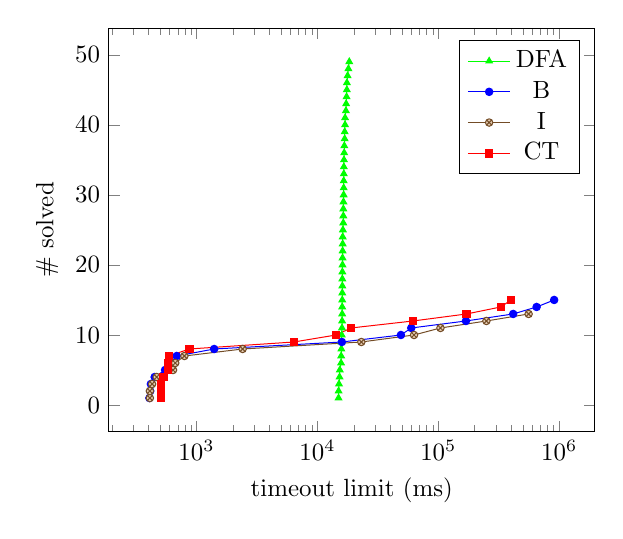
\begin{tikzpicture}[scale=0.9]
      \begin{axis}[
    xmode=log,
    every axis plot/.style={thin},
    xlabel={timeout limit (ms)},
    ylabel={\# solved},
    legend pos=north east
    % table/create on use/cumulative distribution/.style={
    %   create col/expr={\pgfmathaccuma + \thisrow{f(x)}}   
    % }
    ]
    \addplot 
    [mark=triangle*,
    mark size=1.5,
    mark options={solid},
    green] 
    coordinates {
    (14955.640, 1)
(14968.715, 2)
(15081.852, 3)
(15246.230, 4)
(15319.517, 5)
(15694.443, 6)
(15719.960, 7)
(15775.606, 8)
(15786.850, 9)
(15896.231, 10)
(15965.343, 11)
(16005.555, 12)
(16025.117, 13)
(16031.876, 14)
(16045.846, 15)
(16051.370, 16)
(16069.886, 17)
(16072.811, 18)
(16083.237, 19)
(16121.665, 20)
(16136.113, 21)
(16156.801, 22)
(16176.375, 23)
(16178.653, 24)
(16245.676, 25)
(16366.799, 26)
(16378.158, 27)
(16380.892, 28)
(16416.757, 29)
(16478.895, 30)
(16497.038, 31)
(16500.046, 32)
(16533.794, 33)
(16540.436, 34)
(16585.806, 35)
(16652.982, 36)
(16691.128, 37)
(16800.390, 38)
(16810.154, 39)
(16925.261, 40)
(16928.061, 41)
(17203.760, 42)
(17283.698, 43)
(17423.272, 44)
(17512.601, 45)
(17538.616, 46)
(17769.707, 47)
(18045.623, 48)
(18343.375, 49)
    };

    \addplot 
    [blue,
    mark=*,
    mark size=1.5,
    mark options={solid}]
    coordinates {
    (407.759, 1)
(414.434, 2)
(419.216, 3)
(450.778, 4)
(549.394, 5)
(610.163, 6)
(686.273, 7)
(1398.874, 8)
(15928.727, 9)
(49039.533, 10)
(59721.595, 11)
(169215.924, 12)
(415997.085, 13)
(649968.448, 14)
(907521.385, 15)
% (1000382.106, 16)
% (1000387.429, 17)
% (1000388.151, 18)
% (1000388.347, 19)
% (1000390.684, 20)
% (1000395.468, 21)
% (1000398.451, 22)
% (1000400.524, 23)
% (1000400.706, 24)
% (1000401.730, 25)
% (1000401.841, 26)
% (1000403.654, 27)
% (1000403.994, 28)
% (1000404.160, 29)
% (1000404.725, 30)
% (1000405.072, 31)
% (1000406.271, 32)
% (1000406.289, 33)
% (1000408.137, 34)
% (1000409.168, 35)
% (1000409.171, 36)
% (1000409.900, 37)
% (1000409.919, 38)
% (1000410.346, 39)
% (1000411.211, 40)
% (1000412.274, 41)
% (1000412.434, 42)
% (1000413.669, 43)
% (1000413.697, 44)
% (1000413.893, 45)
% (1000415.159, 46)
% (1000415.655, 47)
% (1000416.766, 48)
% (1000417.147, 49)
    };

    \addplot [brown!60!black,
    mark options={fill=brown!40},
    mark=otimes*,
    mark size=1.5]
    coordinates {
    (411.425, 1)
(411.643, 2)
(429.292, 3)
(468.693, 4)
(639.628, 5)
(667.122, 6)
(794.022, 7)
(2406.553, 8)
(23078.974, 9)
(62957.355, 10)
(104153.981, 11)
(249841.503, 12)
(558201.118, 13)
% (1000388.044, 14)
% (1000402.477, 15)
% (1000403.436, 16)
% (1000404.783, 17)
% (1000405.378, 18)
% (1000405.704, 19)
% (1000406.897, 20)
% (1000406.968, 21)
% (1000407.434, 22)
% (1000407.466, 23)
% (1000408.430, 24)
% (1000410.331, 25)
% (1000411.890, 26)
% (1000412.483, 27)
% (1000413.619, 28)
% (1000413.815, 29)
% (1000414.349, 30)
% (1000417.491, 31)
% (1000417.949, 32)
% (1000418.050, 33)
% (1000418.110, 34)
% (1000419.106, 35)
% (1000421.213, 36)
% (1000425.194, 37)
% (1000425.968, 38)
% (1000429.409, 39)
% (1000430.069, 40)
% (1000430.274, 41)
% (1000431.550, 42)
% (1000431.958, 43)
% (1000434.278, 44)
% (1000435.376, 45)
% (1000437.954, 46)
% (1000465.864, 47)
% (1000470.438, 48)
% (1000485.931, 49)
    };

    \addplot 
    [red,
    mark size=1.5,
    mark=square*]
    coordinates {
    (508.071, 1)
(509.196, 2)
(510.855, 3)
(534.756, 4)
(578.458, 5)
(581.294, 6)
(592.155, 7)
(871.362, 8)
(6376.939, 9)
(14282.674, 10)
(18970.185, 11)
(61800.545, 12)
(171097.990, 13)
(328543.590, 14)
(399691.539, 15)
% (1000508.452, 16)
% (1000510.576, 17)
% (1000511.037, 18)
% (1000515.800, 19)
% (1000516.296, 20)
% (1000522.133, 21)
% (1000522.266, 22)
% (1000527.510, 23)
% (1000527.510, 24)
% (1000530.273, 25)
% (1000530.582, 26)
% (1000535.684, 27)
% (1000536.663, 28)
% (1000538.258, 29)
% (1000538.752, 30)
% (1000538.821, 31)
% (1000539.927, 32)
% (1000542.929, 33)
% (1000543.075, 34)
% (1000543.682, 35)
% (1000543.865, 36)
% (1000547.730, 37)
% (1000548.803, 38)
% (1000549.065, 39)
% (1000549.762, 40)
% (1000552.156, 41)
% (1000552.610, 42)
% (1000560.835, 43)
% (1000562.921, 44)
% (1000565.715, 45)
% (1000567.437, 46)
% (1000570.129, 47)
% (1000576.494, 48)
% (1000627.930, 49)
    };
    \legend{DFA,B,I,CT}
  \end{axis}

    \end{tikzpicture}
    \vfill
    \caption{\textbf{Mod Renault}.}
    \vspace{\baselineskip}
  \end{minipage}\qquad
  \begin{minipage}[b][10cm][s]{0.45\textwidth}
    \centering
    \vfill
    \begin{tikzpicture}[scale=0.9]
      \begin{axis}[
    xmode=log,
    every axis plot/.style={thin},
    xlabel={timeout limit (ms)},
    ylabel={\% solved},
    legend style={at={(0.5,-0.30)},
      anchor=north,legend columns=-1},
    % legend pos=south east,
    cycle list/Set1-6,
            % define fill color for the marker
            mark list fill={.!75!white},
            mark options={solid,scale=0.9},
            cycle multiindex* list={
                Set1-6
                    \nextlist
                [3 of]linestyles
                    \nextlist
                very thick
                \nextlist
                mark=o,
                mark=*,
                mark=square,
                mark=triangle,
                mark=+
            },
    ]

    \addplot
    coordinates {
      (550, 7)
      (1420, 13)
      (2180, 19)
      (2460, 25)
      (4050, 32)
      (11860, 38)
      (37590, 44)
      (42030, 50)
      (51040, 57)
      (744510, 63)
      (828510, 69)
      (921350, 75)
      
    };
    \addplot
    coordinates {
      (730, 7)
      (2790, 13)
      (2950, 19)
      (9950, 25)
      (22390, 32)
      (55820, 38)
      (79890, 44)
      (247070, 50)
      
    };
    \addplot
    coordinates {
      (720, 7)
      (2880, 13)
      (4460, 19)
      (11570, 25)
      (21880, 32)
      (80590, 38)
      (84470, 44)
      (276470, 50)
      
    };
    \addplot
    coordinates {
      (140, 7)
      (210, 13)
      (680, 19)
      (1410, 25)
      (1760, 32)
      (2610, 38)
      (23590, 44)
      (29830, 50)
      (49050, 57)
      (474090, 63)
      (606460, 69)
      
    };
    

    \legend{ DFA, B, I, \textbf{CT} }
  \end{axis}

    \end{tikzpicture}
    \vfill
    \caption{\textbf{Pigeons Plus}.}
    \vspace{\baselineskip}
  \end{minipage}\qquad
\end{figure}

\begin{figure}
  \begin{minipage}[b][10cm][s]{0.45\textwidth}
    \centering
    \vfill
    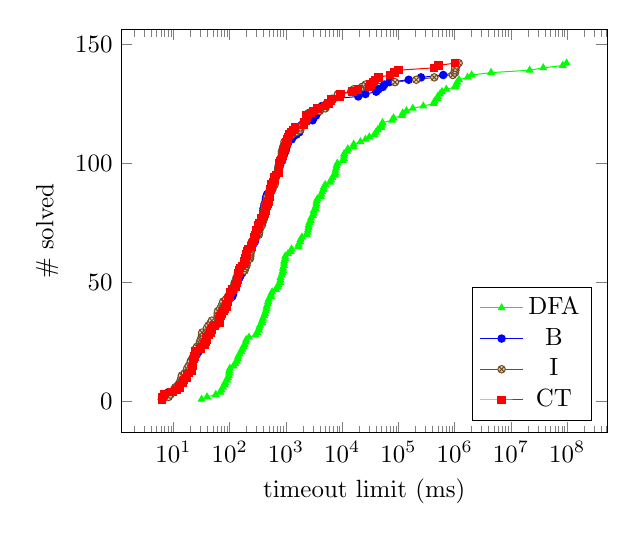
\begin{tikzpicture}[scale=0.9]
      \begin{axis}[
    xmode=log,
    every axis plot/.style={thin},
    xlabel={timeout limit (ms)},
    ylabel={\# solved},
    legend pos=south east
    % table/create on use/cumulative distribution/.style={
    %   create col/expr={\pgfmathaccuma + \thisrow{f(x)}}   
    % }
    ]
    \addplot 
    [mark=triangle*,
    mark size=1.5,
    mark options={solid},
    green] 
    coordinates {
    (31.696, 1)
(39.559, 2)
(56.508, 3)
(68.178, 4)
(70.931, 5)
(75.984, 6)
(81.689, 7)
(82.437, 8)
(90.551, 9)
(92.696, 10)
(96.318, 11)
(97.489, 12)
(98.251, 13)
(100.928, 14)
(116.739, 15)
(124.823, 16)
(132.967, 17)
(139.159, 18)
(141.636, 19)
(149.509, 20)
(161.219, 21)
(165.144, 22)
(176.745, 23)
(182.586, 24)
(193.826, 25)
(196.443, 26)
(220.596, 27)
(287.801, 28)
(307.637, 29)
(331.351, 30)
(335.110, 31)
(344.194, 32)
(377.529, 33)
(378.932, 34)
(389.655, 35)
(410.350, 36)
(423.248, 37)
(438.655, 38)
(450.859, 39)
(454.186, 40)
(475.260, 41)
(483.019, 42)
(493.122, 43)
(544.266, 44)
(544.377, 45)
(568.390, 46)
(658.959, 47)
(704.627, 48)
(733.115, 49)
(790.697, 50)
(796.819, 51)
(799.668, 52)
(839.106, 53)
(863.117, 54)
(884.469, 55)
(886.545, 56)
(921.009, 57)
(927.374, 58)
(928.500, 59)
(970.121, 60)
(970.451, 61)
(1084.311, 62)
(1214.035, 63)
(1256.732, 64)
(1667.050, 65)
(1679.067, 66)
(1790.603, 67)
(1813.082, 68)
(1923.256, 69)
(2334.693, 70)
(2424.581, 71)
(2460.778, 72)
(2524.488, 73)
(2535.289, 74)
(2608.483, 75)
(2727.527, 76)
(2790.777, 77)
(3010.831, 78)
(3089.396, 79)
(3100.186, 80)
(3342.097, 81)
(3421.319, 82)
(3476.286, 83)
(3498.766, 84)
(3603.983, 85)
(4152.208, 86)
(4252.733, 87)
(4414.005, 88)
(4619.485, 89)
(4703.303, 90)
(4995.143, 91)
(6104.482, 92)
(6327.657, 93)
(6680.221, 94)
(7451.205, 95)
(7524.283, 96)
(7577.742, 97)
(7815.366, 98)
(7963.806, 99)
(8190.616, 100)
(10239.338, 101)
(10646.387, 102)
(10743.772, 103)
(10816.354, 104)
(12183.647, 105)
(12608.953, 106)
(15986.466, 107)
(16016.047, 108)
(21085.457, 109)
(25840.612, 110)
(30330.074, 111)
(37303.992, 112)
(39784.632, 113)
(42867.757, 114)
(49654.939, 115)
(49896.816, 116)
(51937.811, 117)
(76626.715, 118)
(81762.693, 119)
(116690.715, 120)
(118979.114, 121)
(138352.575, 122)
(179596.690, 123)
(275896.959, 124)
(422494.853, 125)
(435710.733, 126)
(490650.459, 127)
(500154.998, 128)
(546044.177, 129)
(592457.334, 130)
(707795.890, 131)
(1014847.682, 132)
(1051973.108, 133)
(1109712.990, 134)
(1188811.633, 135)
(1691073.549, 136)
(1998815.209, 137)
(4412151.304, 138)
(21464315.090, 139)
(37446981.305, 140)
(83163795.720, 141)
(97236200.525, 142)
    };

    \addplot 
    [blue,
    mark=*,
    mark size=1.5,
    mark options={solid}]
    coordinates {
    (6.266, 1)
(6.620, 2)
(7.191, 3)
(8.174, 4)
(10.291, 5)
(11.099, 6)
(12.126, 7)
(13.714, 8)
(14.201, 9)
(17.122, 10)
(17.173, 11)
(18.736, 12)
(19.358, 13)
(19.989, 14)
(20.187, 15)
(20.291, 16)
(20.437, 17)
(21.788, 18)
(22.787, 19)
(26.326, 20)
(28.086, 21)
(28.501, 22)
(30.269, 23)
(30.327, 24)
(31.429, 25)
(32.957, 26)
(35.312, 27)
(37.683, 28)
(42.027, 29)
(44.010, 30)
(45.270, 31)
(57.413, 32)
(58.136, 33)
(60.287, 34)
(63.612, 35)
(64.377, 36)
(70.203, 37)
(71.636, 38)
(74.510, 39)
(81.417, 40)
(81.885, 41)
(86.850, 42)
(98.379, 43)
(110.554, 44)
(114.955, 45)
(116.342, 46)
(116.797, 47)
(117.697, 48)
(127.569, 49)
(128.638, 50)
(132.319, 51)
(149.619, 52)
(156.554, 53)
(167.748, 54)
(171.866, 55)
(177.579, 56)
(186.974, 57)
(188.731, 58)
(197.746, 59)
(206.427, 60)
(212.854, 61)
(223.093, 62)
(234.349, 63)
(237.887, 64)
(249.281, 65)
(261.335, 66)
(279.625, 67)
(282.633, 68)
(287.627, 69)
(297.860, 70)
(315.101, 71)
(322.909, 72)
(331.748, 73)
(351.193, 74)
(352.948, 75)
(363.872, 76)
(366.739, 77)
(390.571, 78)
(395.284, 79)
(397.359, 80)
(399.002, 81)
(410.756, 82)
(418.082, 83)
(436.759, 84)
(439.198, 85)
(447.297, 86)
(462.840, 87)
(504.442, 88)
(543.477, 89)
(559.175, 90)
(566.240, 91)
(601.149, 92)
(619.715, 93)
(652.612, 94)
(657.839, 95)
(715.983, 96)
(731.157, 97)
(752.783, 98)
(784.906, 99)
(794.121, 100)
(856.340, 101)
(862.438, 102)
(901.933, 103)
(927.762, 104)
(979.127, 105)
(1000.759, 106)
(1023.428, 107)
(1067.513, 108)
(1074.968, 109)
(1265.279, 110)
(1331.799, 111)
(1538.059, 112)
(1731.374, 113)
(1737.023, 114)
(1790.519, 115)
(1895.419, 116)
(2041.525, 117)
(2975.267, 118)
(3105.441, 119)
(3430.058, 120)
(3574.657, 121)
(3985.434, 122)
(4137.262, 123)
(4364.834, 124)
(5314.336, 125)
(6189.835, 126)
(6463.719, 127)
(19294.688, 128)
(25874.502, 129)
(40075.340, 130)
(44076.314, 131)
(52831.470, 132)
(56117.125, 133)
(69049.283, 134)
(151946.681, 135)
(251788.612, 136)
(624723.233, 137)
(1006224.760, 138)
(1024927.746, 139)
(1025126.900, 140)
(1051096.785, 141)
(1054709.554, 142)
    };

    \addplot [brown!60!black,
    mark options={fill=brown!40},
    mark=otimes*,
    mark size=1.5]
    coordinates {
    (6.225, 1)
(8.252, 2)
(8.866, 3)
(8.903, 4)
(10.276, 5)
(10.793, 6)
(12.246, 7)
(12.967, 8)
(13.482, 9)
(13.873, 10)
(14.125, 11)
(15.975, 12)
(17.388, 13)
(17.590, 14)
(18.641, 15)
(20.043, 16)
(20.476, 17)
(21.613, 18)
(23.615, 19)
(24.164, 20)
(24.372, 21)
(24.882, 22)
(26.053, 23)
(29.400, 24)
(29.513, 25)
(30.549, 26)
(31.898, 27)
(32.205, 28)
(32.366, 29)
(39.353, 30)
(39.524, 31)
(42.127, 32)
(45.853, 33)
(48.185, 34)
(60.297, 35)
(60.940, 36)
(61.286, 37)
(61.970, 38)
(67.684, 39)
(71.354, 40)
(74.374, 41)
(76.755, 42)
(86.492, 43)
(92.532, 44)
(102.074, 45)
(107.118, 46)
(110.458, 47)
(119.452, 48)
(120.692, 49)
(122.537, 50)
(130.211, 51)
(131.757, 52)
(139.069, 53)
(139.341, 54)
(184.184, 55)
(187.471, 56)
(198.576, 57)
(201.040, 58)
(207.945, 59)
(229.958, 60)
(232.188, 61)
(233.976, 62)
(239.163, 63)
(240.688, 64)
(241.932, 65)
(243.311, 66)
(245.547, 67)
(265.954, 68)
(292.029, 69)
(328.546, 70)
(334.072, 71)
(336.358, 72)
(350.752, 73)
(375.324, 74)
(379.234, 75)
(396.967, 76)
(401.683, 77)
(401.895, 78)
(405.570, 79)
(411.227, 80)
(417.570, 81)
(419.966, 82)
(421.977, 83)
(456.664, 84)
(458.121, 85)
(467.458, 86)
(514.809, 87)
(537.183, 88)
(573.529, 89)
(585.083, 90)
(628.983, 91)
(629.151, 92)
(638.579, 93)
(655.494, 94)
(683.596, 95)
(719.854, 96)
(720.103, 97)
(726.177, 98)
(743.018, 99)
(776.859, 100)
(788.068, 101)
(801.667, 102)
(840.869, 103)
(844.819, 104)
(845.660, 105)
(882.665, 106)
(896.694, 107)
(936.968, 108)
(941.257, 109)
(1025.243, 110)
(1127.272, 111)
(1290.616, 112)
(1527.467, 113)
(1798.817, 114)
(1803.072, 115)
(1966.245, 116)
(2089.371, 117)
(2225.216, 118)
(2378.815, 119)
(2497.087, 120)
(2503.823, 121)
(3943.794, 122)
(5004.718, 123)
(5143.946, 124)
(5663.752, 125)
(6369.410, 126)
(6913.053, 127)
(8260.886, 128)
(8382.946, 129)
(14367.240, 130)
(16013.595, 131)
(22433.224, 132)
(26100.534, 133)
(86936.175, 134)
(206857.036, 135)
(432302.057, 136)
(923791.300, 137)
(1001275.049, 138)
(1005552.392, 139)
(1024252.398, 140)
(1082346.127, 141)
(1174868.682, 142)
    };

    \addplot 
    [red,
    mark size=1.5,
    mark=square*]
    coordinates {
    (6.328, 1)
(6.344, 2)
(6.785, 3)
(9.703, 4)
(11.389, 5)
(12.785, 6)
(13.199, 7)
(14.710, 8)
(15.330, 9)
(17.053, 10)
(17.466, 11)
(18.730, 12)
(21.191, 13)
(21.458, 14)
(22.190, 15)
(22.321, 16)
(22.429, 17)
(23.230, 18)
(23.566, 19)
(24.810, 20)
(24.843, 21)
(30.529, 22)
(31.162, 23)
(35.615, 24)
(37.410, 25)
(38.475, 26)
(38.831, 27)
(43.209, 28)
(45.793, 29)
(47.775, 30)
(48.066, 31)
(53.755, 32)
(65.633, 33)
(66.267, 34)
(66.798, 35)
(69.198, 36)
(73.621, 37)
(77.636, 38)
(83.309, 39)
(87.127, 40)
(87.800, 41)
(92.901, 42)
(93.082, 43)
(98.471, 44)
(101.548, 45)
(102.853, 46)
(112.950, 47)
(126.755, 48)
(126.916, 49)
(133.777, 50)
(136.483, 51)
(139.301, 52)
(141.708, 53)
(142.901, 54)
(147.720, 55)
(151.267, 56)
(167.047, 57)
(180.053, 58)
(185.002, 59)
(192.458, 60)
(199.346, 61)
(200.444, 62)
(205.194, 63)
(211.032, 64)
(245.046, 65)
(247.635, 66)
(258.985, 67)
(273.140, 68)
(274.226, 69)
(289.992, 70)
(293.258, 71)
(296.666, 72)
(320.259, 73)
(325.794, 74)
(331.950, 75)
(359.459, 76)
(369.740, 77)
(401.942, 78)
(428.598, 79)
(439.186, 80)
(443.919, 81)
(451.155, 82)
(465.721, 83)
(486.636, 84)
(496.533, 85)
(507.498, 86)
(509.344, 87)
(518.391, 88)
(534.298, 89)
(549.969, 90)
(554.731, 91)
(594.595, 92)
(623.445, 93)
(624.194, 94)
(658.888, 95)
(748.721, 96)
(754.742, 97)
(754.776, 98)
(757.089, 99)
(766.244, 100)
(789.618, 101)
(856.352, 102)
(878.697, 103)
(882.688, 104)
(885.633, 105)
(948.909, 106)
(961.811, 107)
(1025.381, 108)
(1027.979, 109)
(1068.881, 110)
(1096.069, 111)
(1141.179, 112)
(1263.836, 113)
(1363.480, 114)
(1444.963, 115)
(2086.545, 116)
(2104.289, 117)
(2266.072, 118)
(2315.715, 119)
(2337.155, 120)
(2809.498, 121)
(3062.328, 122)
(3613.655, 123)
(4962.131, 124)
(5757.448, 125)
(6278.281, 126)
(6458.606, 127)
(9074.926, 128)
(9388.538, 129)
(15237.846, 130)
(19012.640, 131)
(29844.102, 132)
(32057.652, 133)
(36009.393, 134)
(38516.958, 135)
(44360.448, 136)
(70712.723, 137)
(84815.013, 138)
(99208.278, 139)
(426595.818, 140)
(513749.533, 141)
(1012388.065, 142)
    };
    \legend{DFA,B,I,CT}
  \end{axis}

    \end{tikzpicture}
    \vfill
    \caption{\textbf{Nonograms}.}
    \vspace{\baselineskip}
  \end{minipage}\qquad
  \begin{minipage}[b][10cm][s]{0.45\textwidth}
    \centering
    \vfill
    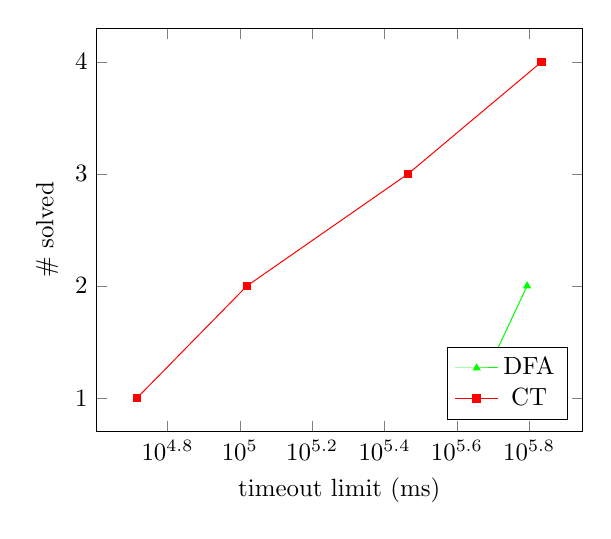
\begin{tikzpicture}[scale=0.9]
      \begin{axis}[
    xmode=log,
    every axis plot/.style={thin},
    xlabel={timeout limit (ms)},
    ylabel={\# solved},
    legend pos=south east
    % table/create on use/cumulative distribution/.style={
    %   create col/expr={\pgfmathaccuma + \thisrow{f(x)}}   
    % }
    ]
    \addplot 
    [mark=triangle*,
    mark size=1.5,
    mark options={solid},
    green] 
    coordinates {
    (445273.296, 1)
(622414.790, 2)
% (1031281.648, 3)
% (1073752.509, 4)
% (1077338.303, 5)
% (1078117.880, 6)
% (1078636.961, 7)
% (1079178.894, 8)
% (1079839.216, 9)
% (1080840.349, 10)
% (1082059.397, 11)
% (1083648.155, 12)
% (1083902.339, 13)
% (1083988.269, 14)
% (1084069.534, 15)
% (1084396.676, 16)
% (1085666.524, 17)
% (1089495.967, 18)
% (1091132.921, 19)
% (1091433.340, 20)
% (1092057.252, 21)
% (1093916.092, 22)
% (1094177.223, 23)
% (1114453.122, 24)
% (1115067.373, 25)
    };

%     \addplot 
%     [blue,
%     mark=*,
%     mark size=1.5,
%     mark options={solid}]
%     coordinates {
%     (1004672.786, 1)
% (1004695.224, 2)
% (1004696.645, 3)
% (1004718.463, 4)
% (1004738.023, 5)
% (1004743.967, 6)
% (1004751.151, 7)
% (1004765.567, 8)
% (1004781.515, 9)
% (1004797.803, 10)
% (1004816.640, 11)
% (1004820.096, 12)
% (1004835.673, 13)
% (1004864.792, 14)
% (1004881.537, 15)
% (1004913.526, 16)
% (1004920.059, 17)
% (1004929.625, 18)
% (1004958.448, 19)
% (1004996.508, 20)
% (1005007.752, 21)
% (1005029.139, 22)
% (1005067.535, 23)
% (1005104.606, 24)
% (1040982.750, 25)
%     };

%     \addplot [brown!60!black,
%     mark options={fill=brown!40},
%     mark=otimes*,
%     mark size=1.5]
%     coordinates {
%     (1004653.569, 1)
% (1004695.464, 2)
% (1004715.665, 3)
% (1004725.629, 4)
% (1004729.598, 5)
% (1004736.757, 6)
% (1004768.906, 7)
% (1004774.513, 8)
% (1004800.095, 9)
% (1004877.671, 10)
% (1004885.444, 11)
% (1004924.289, 12)
% (1004954.273, 13)
% (1004976.220, 14)
% (1005012.748, 15)
% (1005016.479, 16)
% (1005025.501, 17)
% (1005059.309, 18)
% (1005081.774, 19)
% (1005131.686, 20)
% (1005177.022, 21)
% (1005199.107, 22)
% (1005247.884, 23)
% (1005272.462, 24)
% (1103825.908, 25)
%     };

    \addplot 
    [red,
    mark size=1.5,
    mark=square*]
    coordinates {
    (51933.780, 1)
(104573.439, 2)
(291800.057, 3)
(683133.039, 4)
% (1006259.610, 5)
% (1006270.822, 6)
% (1006282.419, 7)
% (1006303.104, 8)
% (1006319.339, 9)
% (1006423.422, 10)
% (1006449.607, 11)
% (1006459.928, 12)
% (1006499.500, 13)
% (1006510.783, 14)
% (1006510.952, 15)
% (1006511.373, 16)
% (1006567.036, 17)
% (1006579.356, 18)
% (1006588.135, 19)
% (1006591.883, 20)
% (1006659.196, 21)
% (1006817.280, 22)
% (1006986.645, 23)
% (1012355.582, 24)
% (1025624.781, 25)
    };
    \legend{DFA,CT}
  \end{axis}

    \end{tikzpicture}
    \vfill
    \caption{\textbf{MDD 05}.}
    \vspace{\baselineskip}
  \end{minipage}\qquad
\end{figure}

\clearpage

\begin{figure}
  \begin{minipage}[b][10cm][s]{.45\textwidth}
     \centering
    \vfill
    \begin{tikzpicture}[scale=0.9]
      \begin{axis}[
    xmode=log,
    every axis plot/.style={thin},
    xlabel={timeout limit (ms)},
    ylabel={\% solved},
    legend pos=south east,
    cycle list/Set1-6,
            % define fill color for the marker
            mark list fill={.!75!white},
            mark options={solid},
            cycle multiindex* list={
                Set1-6
                    \nextlist
                [3 of]linestyles
                    \nextlist
                very thick
                \nextlist
                mark=o,
                mark=*,
                mark=square,
                mark=triangle,
                mark=+
            },
    ]

    \addplot
    coordinates {
      (5500, 10)
      (16070, 20)
      (16630, 30)
      (17890, 40)
      (35390, 50)
      (57330, 60)
      (69990, 70)
      (101460, 80)
      (169980, 90)
      (453800, 100)
      
    };
    \addplot
    coordinates {
      (2230, 10)
      (5650, 20)
      (6980, 30)
      (8620, 40)
      (21360, 50)
      (25040, 60)
      (42030, 70)
      (56640, 80)
      (61450, 90)
      (253650, 100)
      
    };
    \addplot
    coordinates {
      (3120, 10)
      (9240, 20)
      (10460, 30)
      (12500, 40)
      (31710, 50)
      (38200, 60)
      (61930, 70)
      (82230, 80)
      (95830, 90)
      (382920, 100)
      
    };
    \addplot
    coordinates {
      (570, 10)
      (1250, 20)
      (1410, 30)
      (1570, 40)
      (3500, 50)
      (3990, 60)
      (6250, 70)
      (8860, 80)
      (10050, 90)
      (42870, 100)
      
    };
    

    \legend{ DFA, B, I, \textbf{CT} }
  \end{axis}

    \end{tikzpicture}    
    \vfill
    \caption{\textbf{Rands JC2500.}}
    \vspace{\baselineskip}
  \end{minipage}\qquad
  \begin{minipage}[b][10cm][s]{.45\textwidth}
    \centering
    \vfill
    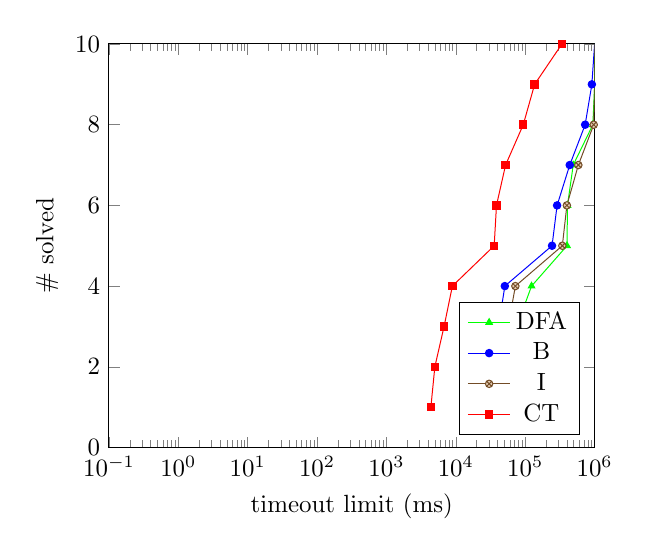
\begin{tikzpicture}[scale=0.9]
      \begin{axis}[
    xmode=log,
    ymin=0,ymax=10,
    xmin=0.1, xmax=1000000,
    every axis plot/.style={thin},
    xlabel={timeout limit (ms)},
    ylabel={\# solved},
    legend pos=south east
    % table/create on use/cumulative distribution/.style={
    %   create col/expr={\pgfmathaccuma + \thisrow{f(x)}}   
    % }
    ]
    \addplot 
    [mark=triangle*,
    mark size=1.5,
    mark options={solid},
    green] 
    coordinates {
    (37271.407, 1)
(63329.760, 2)
(75340.967, 3)
(123361.614, 4)
(400331.140, 5)
(406374.082, 6)
(491965.258, 7)
(943701.318, 8)
(1003127.715, 9)
(1003191.173, 10)
    };

    \addplot 
    [blue,
    mark=*,
    mark size=1.5,
    mark options={solid}]
    coordinates {
    (23487.263, 1)
(31493.067, 2)
(41324.456, 3)
(50843.172, 4)
(243499.863, 5)
(288078.384, 6)
(438078.025, 7)
(731291.713, 8)
(912991.209, 9)
(1000435.280, 10)
    };

    \addplot [brown!60!black,
    mark options={fill=brown!40},
    mark=otimes*,
    mark size=1.5]
    coordinates {
    (31721.470, 1)
(45760.945, 2)
(56699.417, 3)
(72142.510, 4)
(342690.713, 5)
(398501.909, 6)
(583027.925, 7)
(971126.357, 8)
(1000434.235, 9)
(1000435.846, 10)
    };

    \addplot 
    [red,
    mark size=1.5,
    mark=square*]
    coordinates {
    (4367.654, 1)
(4983.151, 2)
(6770.036, 3)
(8914.062, 4)
(35712.233, 5)
(38524.930, 6)
(52111.274, 7)
(93677.132, 8)
(136706.431, 9)
(338099.921, 10)
    };
    \legend{DFA,B,I,CT}
  \end{axis}

    \end{tikzpicture}
    \vfill
    \caption{\textbf{Rands JC5000.}}
    \vspace{\baselineskip}
  \end{minipage}\qquad
\end{figure}

\begin{figure}
    \begin{minipage}[b][10cm][s]{.45\textwidth}
    \centering
    \vfill
    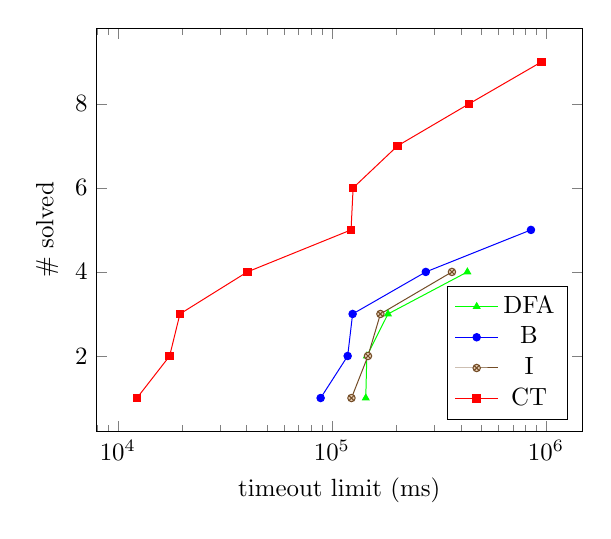
\begin{tikzpicture}[scale=0.9]
      \begin{axis}[
    xmode=log,
    every axis plot/.style={thin},
    xlabel={timeout limit (ms)},
    ylabel={\# solved},
    legend pos=south east
    % table/create on use/cumulative distribution/.style={
    %   create col/expr={\pgfmathaccuma + \thisrow{f(x)}}   
    % }
    ]
    \addplot 
    [mark=triangle*,
    mark size=1.5,
    mark options={solid},
    green] 
    coordinates {
    (143986.214, 1)
(145624.128, 2)
(182844.931, 3)
(429527.079, 4)
% (1004920.333, 5)
% (1005091.406, 6)
% (1005121.020, 7)
% (1005141.458, 8)
% (1005180.694, 9)
% (1005181.896, 10)
    };

    \addplot 
    [blue,
    mark=*,
    mark size=1.5,
    mark options={solid}]
    coordinates {
    (88610.730, 1)
(118513.380, 2)
(124991.902, 3)
(274645.919, 4)
(851285.302, 5)
% (1000662.235, 6)
% (1000665.157, 7)
% (1000667.124, 8)
% (1000679.084, 9)
% (1000680.879, 10)
    };

    \addplot [brown!60!black,
    mark options={fill=brown!40},
    mark=otimes*,
    mark size=1.5]
    coordinates {
    (123456.088, 1)
(147458.027, 2)
(168559.303, 3)
(363926.326, 4)
% (1000644.518, 5)
% (1000648.628, 6)
% (1000660.653, 7)
% (1000663.644, 8)
% (1000669.943, 9)
% (1000672.172, 10)
    };

    \addplot 
    [red,
    mark size=1.5,
    mark=square*]
    coordinates {
    (12283.482, 1)
(17462.103, 2)
(19503.895, 3)
(40266.047, 4)
(122893.209, 5)
(125673.584, 6)
(202682.066, 7)
(437565.193, 8)
(955387.007, 9)
%(1000911.643, 10)
    };
    \legend{DFA,B,I,CT}
  \end{axis}

    \end{tikzpicture}
    \vfill
    \caption{\textbf{Rands JC7500}.}
    \vspace{\baselineskip}
  \end{minipage}\qquad
  \begin{minipage}[b][10cm][s]{.45\textwidth}
    \centering
    \vfill
    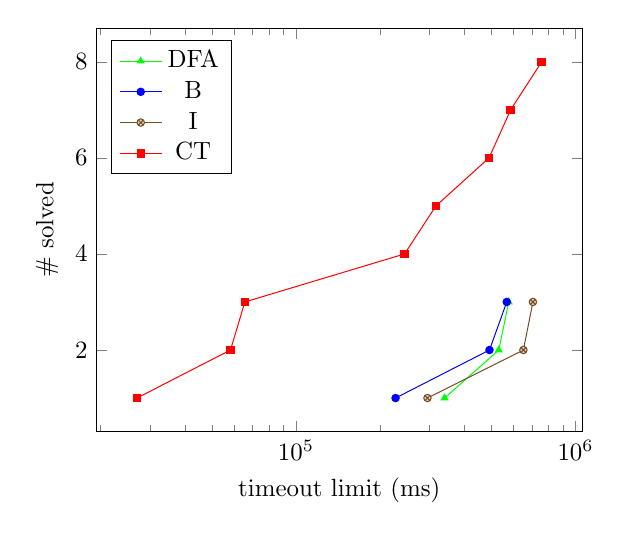
\begin{tikzpicture}[scale=0.9]
      \begin{axis}[
    xmode=log,
    every axis plot/.style={thin},
    xlabel={timeout limit (ms)},
    ylabel={\# solved},
    legend pos=north west
    % table/create on use/cumulative distribution/.style={
    %   create col/expr={\pgfmathaccuma + \thisrow{f(x)}}   
    % }
    ]
    \addplot 
    [mark=triangle*,
    mark size=1.5,
    mark options={solid},
    green] 
    coordinates {
    (339960.449, 1)
(531357.500, 2)
(576758.002, 3)
% (1006830.253, 4)
% (1006953.686, 5)
% (1006987.278, 6)
% (1007012.182, 7)
% (1007040.479, 8)
% (1007166.422, 9)
% (1007385.382, 10)
    };

    \addplot 
    [blue,
    mark=*,
    mark size=1.5,
    mark options={solid}]
    coordinates {
    (227052.199, 1)
(492242.811, 2)
(567372.313, 3)
% (1000877.234, 4)
% (1000889.042, 5)
% (1000892.874, 6)
% (1000895.207, 7)
% (1000911.856, 8)
% (1000913.878, 9)
% (1000928.789, 10)
    };

    \addplot [brown!60!black,
    mark options={fill=brown!40},
    mark=otimes*,
    mark size=1.5]
    coordinates {
    (295287.152, 1)
(650810.991, 2)
(703794.608, 3)
% (1000887.426, 4)
% (1000895.815, 5)
% (1000897.600, 6)
% (1000901.551, 7)
% (1000905.923, 8)
% (1000907.888, 9)
% (1000913.436, 10)
    };

    \addplot 
    [red,
    mark size=1.5,
    mark=square*]
    coordinates {
    (26984.703, 1)
(58304.179, 2)
(65624.179, 3)
(244616.117, 4)
(316746.918, 5)
(490346.243, 6)
(586068.768, 7)
(756641.057, 8)
%(1001171.576, 9)
%(1001192.839, 10)
    };
    \legend{DFA,B,I,CT}
  \end{axis}

    \end{tikzpicture}
    \vfill
    \caption{\textbf{Rands JC10000}.}
    \vspace{\baselineskip}
  \end{minipage}\qquad

\end{figure}

\clearpage

\begin{figure}
  \begin{minipage}[b][10cm][s]{0.45\textwidth}
    \centering
    \vfill
    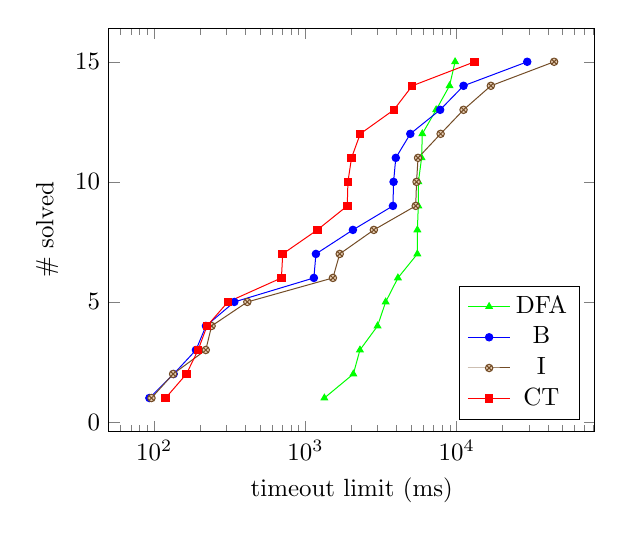
\begin{tikzpicture}[scale=0.9]
      \begin{axis}[
    xmode=log,
    every axis plot/.style={thin},
    xlabel={timeout limit (ms)},
    ylabel={\# solved},
    legend pos=south east
    % table/create on use/cumulative distribution/.style={
    %   create col/expr={\pgfmathaccuma + \thisrow{f(x)}}   
    % }
    ]
    \addplot 
    [mark=triangle*,
    mark size=1.5,
    mark options={solid},
    green] 
    coordinates {
    (1333.406, 1)
(2072.861, 2)
(2291.811, 3)
(2996.127, 4)
(3390.696, 5)
(4085.322, 6)
(5492.735, 7)
(5494.497, 8)
(5573.341, 9)
(5581.970, 10)
(5861.969, 11)
(5923.068, 12)
(7311.924, 13)
(8965.104, 14)
(9758.067, 15)
    };

    \addplot 
    [blue,
    mark=*,
    mark size=1.5,
    mark options={solid}]
    coordinates {
    (92.898, 1)
(134.489, 2)
(188.799, 3)
(219.819, 4)
(338.413, 5)
(1136.522, 6)
(1172.713, 7)
(2058.962, 8)
(3789.293, 9)
(3824.374, 10)
(3956.922, 11)
(4935.345, 12)
(7773.796, 13)
(11094.603, 14)
(29268.417, 15)
    };

    \addplot [brown!60!black,
    mark options={fill=brown!40},
    mark=otimes*,
    mark size=1.5]
    coordinates {
    (95.886, 1)
(133.264, 2)
(219.206, 3)
(239.481, 4)
(412.639, 5)
(1518.706, 6)
(1684.622, 7)
(2831.549, 8)
(5358.480, 9)
(5425.453, 10)
(5551.804, 11)
(7829.008, 12)
(11095.700, 13)
(16823.395, 14)
(44072.919, 15)
    };

    \addplot 
    [red,
    mark size=1.5,
    mark=square*]
    coordinates {
    (118.884, 1)
(163.180, 2)
(195.126, 3)
(223.383, 4)
(307.055, 5)
(693.402, 6)
(707.378, 7)
(1197.949, 8)
(1889.844, 9)
(1908.499, 10)
(2016.541, 11)
(2302.896, 12)
(3841.743, 13)
(5082.583, 14)
(13144.847, 15)
    };
    \legend{DFA,B,I,CT}
  \end{axis}

    \end{tikzpicture}
    \vfill
    \caption{\textbf{TSP 20}.}
    \vspace{\baselineskip}
  \end{minipage}\qquad
  \begin{minipage}[b][10cm][s]{0.45\textwidth}
    \centering
    \vfill
    \begin{tikzpicture}[scale=0.9]
      \begin{axis}[
    xmode=log,
    every axis plot/.style={thin},
    xlabel={timeout limit (ms)},
    ylabel={\% solved},
    legend pos=south east,
    cycle list/Set1-6,
            % define fill color for the marker
            mark list fill={.!75!white},
            mark options={solid},
            cycle multiindex* list={
                Set1-6
                    \nextlist
                [3 of]linestyles
                    \nextlist
                very thick
                \nextlist
                mark=o,
                mark=*,
                mark=square,
                mark=triangle,
                mark=+
            },
    ]

    \addplot
    coordinates {
      (2310, 7)
      (3050, 14)
      (3280, 20)
      (3480, 27)
      (4110, 34)
      (4640, 40)
      (6230, 47)
      (6550, 54)
      (6570, 60)
      (7330, 67)
      (7780, 74)
      (8210, 80)
      (8270, 87)
      (8360, 94)
      (12510, 100)
      
    };
    \addplot
    coordinates {
      (610, 7)
      (820, 14)
      (990, 20)
      (1200, 27)
      (1250, 34)
      (1530, 40)
      (8430, 47)
      (8550, 54)
      (13190, 60)
      (14750, 67)
      (22720, 74)
      (26230, 80)
      (34060, 87)
      (99550, 94)
      (196100, 100)
      
    };
    \addplot
    coordinates {
      (720, 7)
      (1040, 14)
      (1180, 20)
      (1570, 27)
      (1610, 34)
      (2060, 40)
      (11310, 47)
      (12140, 54)
      (17130, 60)
      (19510, 67)
      (31680, 74)
      (37680, 80)
      (47500, 87)
      (136970, 94)
      (261960, 100)
      
    };
    \addplot
    coordinates {
      (400, 7)
      (550, 14)
      (560, 20)
      (630, 27)
      (690, 34)
      (800, 40)
      (3710, 47)
      (3760, 54)
      (5650, 60)
      (5810, 67)
      (9780, 74)
      (10930, 80)
      (13290, 87)
      (43980, 94)
      (77540, 100)
      
    };
    

    \legend{ DFA, B, I, \textbf{CT} }
  \end{axis}

    \end{tikzpicture}
    \vfill
    \caption{\textbf{TSP 25}.}
    \vspace{\baselineskip}
  \end{minipage}\qquad
\end{figure}


\begin{figure}
  \begin{minipage}[b][10cm][s]{0.45\textwidth}
    \centering
    \vfill
    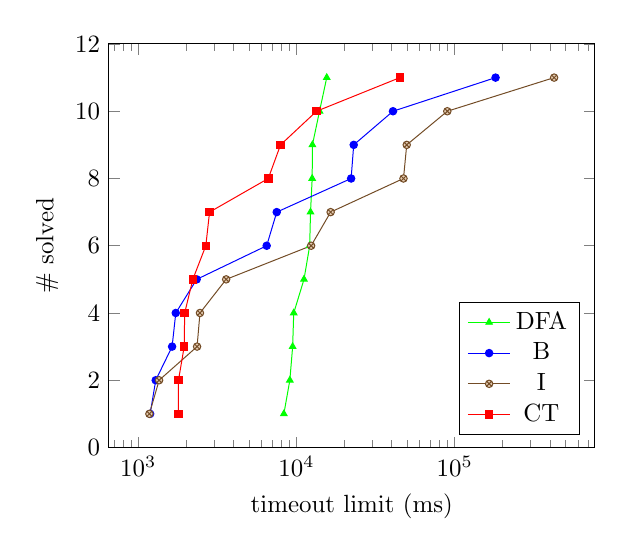
\begin{tikzpicture}[scale=0.9]
      \begin{axis}[
    xmode=log,
    every axis plot/.style={thin},
    xlabel={timeout limit (ms)},
    ylabel={\# solved},
    legend pos=south east
    % table/create on use/cumulative distribution/.style={
    %   create col/expr={\pgfmathaccuma + \thisrow{f(x)}}   
    % }
    ]
    \addplot 
    [mark=triangle*,
    mark size=1.5,
    mark options={solid},
    green] 
    coordinates {
    (8323.942, 1)
(9080.418, 2)
(9457.327, 3)
(9611.154, 4)
(11157.909, 5)
(12122.318, 6)
(12269.578, 7)
(12569.631, 8)
(12613.425, 9)
(13987.860, 10)
(15538.867, 11)
    };

    \addplot 
    [blue,
    mark=*,
    mark size=1.5,
    mark options={solid}]
    coordinates {
    (1188.206, 1)
(1289.021, 2)
(1636.318, 3)
(1725.962, 4)
(2339.887, 5)
(6481.991, 6)
(7504.933, 7)
(22155.924, 8)
(23009.793, 9)
(40756.444, 10)
(181399.438, 11)
    };

    \addplot [brown!60!black,
    mark options={fill=brown!40},
    mark=otimes*,
    mark size=1.5]
    coordinates {
    (1175.718, 1)
(1354.438, 2)
(2353.159, 3)
(2454.453, 4)
(3594.396, 5)
(12379.752, 6)
(16444.353, 7)
(47478.184, 8)
(49773.525, 9)
(89852.322, 10)
(425399.368, 11)
    };

    \addplot 
    [red,
    mark size=1.5,
    mark=square*]
    coordinates {
    (1794.640, 1)
(1795.355, 2)
(1951.150, 3)
(1965.074, 4)
(2212.001, 5)
(2673.018, 6)
(2822.171, 7)
(6633.134, 8)
(7933.220, 9)
(13389.469, 10)
(45079.672, 11)
    };
    \legend{DFA,B,I,CT}
  \end{axis}

    \end{tikzpicture}
    \vfill
    \caption{\textbf{TSP Quat 20}.}
    \vspace{\baselineskip}
  \end{minipage}\qquad
\end{figure}

\clearpage


